\documentclass[a4paper,11pt,oneside,brazilian,
draft=false,twocolumn]{report}%openany,version=last

\setlength{\columnsep}{15pt}
\usepackage{float} 
\usepackage{rotating}
\usepackage{graphicx}
\usepackage{mybook}
\usepackage{fancyhdr} 
\usepackage{pdflscape}
\usepackage{pdfpages} 
\usepackage[toc,page]{appendix}
\usepackage{titlesec}
\usepackage{xcolor}
\usepackage{framed}
\usepackage{titletoc}
\usepackage{longtable}
\usepackage[brazilian]{babel} 
\usepackage{hyperref} 

\newcommand*{\fancychapterstyle}{%
  \titleformat{\chapter} % command
	[block] % shape
	{\bfseries\Large\itshape} % format
	{	\textsc{\LARGE Compilação de relatórios técnicos} 
		\newline \newline  
		\textsc{\Large Capítulo \ \thechapter}
	} % label
	{0.5ex} % sep
	{
    	\rule{\textwidth}{2pt}
    	\vspace{1ex}
    	\centering
    	\huge \textnormal
	} % before-code
	[
		\vspace{-1ex}%
		\rule{\textwidth}{2pt}
		\vfill 
\includegraphics{logo/EMMA-logo}
	] % after-code
}

\newcommand*{\standardchapterstyle}{%
  \titleformat{\chapter}[display]
  {\normalfont\huge\bfseries}{\chaptertitlename\ \thechapter}{20pt}{\Huge}
  \titlespacing*{\chapter}{0pt}{50pt}{40pt}
}
 
\pdfcompresslevel = 9
\oddsidemargin = 31pt
\topmargin = 20pt
\headheight = 12pt
\headsep = 25pt
\textheight = 592pt
\textwidth = 390pt
\marginparsep = 10pt
\marginparwidth = 35pt
\footskip = 30pt
\pagenumbering{gobble}

\begin{document} 
 
\pagenumbering{arabic}  
\begin{titlepage}
	\centering
	
\includegraphics{logo/EMMA-logo}
	\vfill
	{\scshape\LARGE Compilação de Relatórios Técnicos \par}
	\vfill

% Bottom of the page
	{\large \today\par}
\end{titlepage}

% \begin{titlepage}
% 	\centering
% 	\includegraphics[width=0.15\textwidth]{example-image-1x1}\par\vspace{1cm}
% 	{\scshape\LARGE Columbidae University \par}
% 	\vspace{1cm}
% 	{\scshape\Large Final year project\par}
% 	\vspace{1.5cm}
% 	{\huge\bfseries Pigeons love doves\par}
% 	\vspace{2cm}
% 	{\Large\itshape John Birdwatch\par}
% 	\vfill
% 	supervised by\par
% 	Dr.~Mark \textsc{Brown}
% 
% 	\vfill
% 
% % Bottom of the page
% 	{\large \today\par}
% \end{titlepage}




%%******************************************************************************
%%
%% frontpage.tex
%%
%%******************************************************************************
%%
%% Title......: ROSA - Stoplog Inspection
%%
%% Author.....: GSCAR-DFKI
%%
%% Started....: Nov 2013
%%
%% Emails.....: renan028@gmail.com
%%
%% Address....: Universidade Federal do Rio de Janeiro
%%              Caixa Postal 68.504, CEP: 21.945-970
%%              Rio de Janeiro, RJ - Brasil.
%%
%%******************************************************************************


%%******************************************************************************
%% FRONT PAGE
%%******************************************************************************




%%==============================================================================
%% FRONT PAGE CONTENTS
%%==============================================================================
\thispagestyle{empty}

%% Restart page counter.
\setpagecounter{0}

%% Disable page anchor to avoid multiple page number definition warnings.
\hypersetup{pageanchor=false}

\vspace{4cm}

 \textcolor{gray}{Execução:} \\
\\
\begin{minipage}{\textwidth}
	\centering
	
\includegraphics[width=0.3\textwidth]{logo/lead-logo}
    \hspace{0.5cm}
	
\includegraphics[width=0.3\textwidth,
    height=0.2\textwidth,keepaspectratio]{logo/minerva07}
	
\end{minipage}

\vspace{2cm}

\textcolor{gray}{Financiamento: } \\ 
\\
\begin{minipage}{\textwidth}
	\centering
	
	
\includegraphics[width=0.3\textwidth]{logo/esbr-logo}
	
\includegraphics[width=0.3\textwidth]{logo/aneel-logo}

	
\end{minipage}

\vspace{4cm}

\begin{table}[ht!]
	\centering
	\begin{tabular}{r l|l p{12cm} }
		\textcolor{gray}{Projeto} &&& \textbf{\Large EMMA}\\
			&&& \textbf{Metodologia de Revestimento Robótico de turbinas in situ}\\
			&&& \\
		\textcolor{gray}{Título} &&& \textbf{Relatório final das atividades
		realizadas no projeto}\\
		\textcolor{gray}{PD} &&& 6631-0003/2015 \\
		\textcolor{gray}{Contrato} &&& Jirau 09/15\\
		\textcolor{gray}{Coordenador} &&& Ramon Romankevicius Costa \\
		\textcolor{gray}{Gerente} &&& Breno Bellinati de Carvalho \\
		%\textcolor{gray}{Data:} &&& \today \\
	\end{tabular}
\end{table}


\cleardoublepage

%%==============================================================================
%% AUTHORS AND VERSION PAGE
%%==============================================================================

% \thispagestyle{empty}
% 
% %% Restart page counter.
% \setpagecounter{0}
% 
% \begin{center}
%   %% Version section. --------------------------------------------------------
% 
%   
%  \vfill
%   %% Project section. --------------------------------------------------------
% 
% 
%   %% Authors section. --------------------------------------------------------
% 
%   {\LARGE Versão}
%   \vspace{0.50cm}
% 
% 
% 
%   \begin{center}
%     \begin{tabular}{| l | l | l |}
%     \hline
%    	 Versão 					& Autor			 & Descrição 	 \\ \hline
%    	 1.0 		& Renan  	& Implementação Inicial\\			
%     
%     \hline 
%     \end{tabular}
% \end{center}
% 
% 
% 
% 
% 
% 
% \end{center}
% 
% \newpage

%% Enable page anchor again.
\hypersetup{pageanchor=true}



\tableofcontents

\fancychapterstyle

\chapter{Resumo gerencial}\label{chap::resumo}

\section{Descrição da Inovação}

A inovação no projeto EMMA é utilizar a robótica para realizar reparo e
revestimento in situ em pás de turbinas de hidroelétricas, ou seja, sem precisar
desinstalar e remover as pás. A metodologia do processo é iniciada com o
ensecamento e entrada do corpo técnico ao circuito hidráulico. A metodologia
desenvolvida segue como explicado pelas imagens.

\begin{figure}[H] 
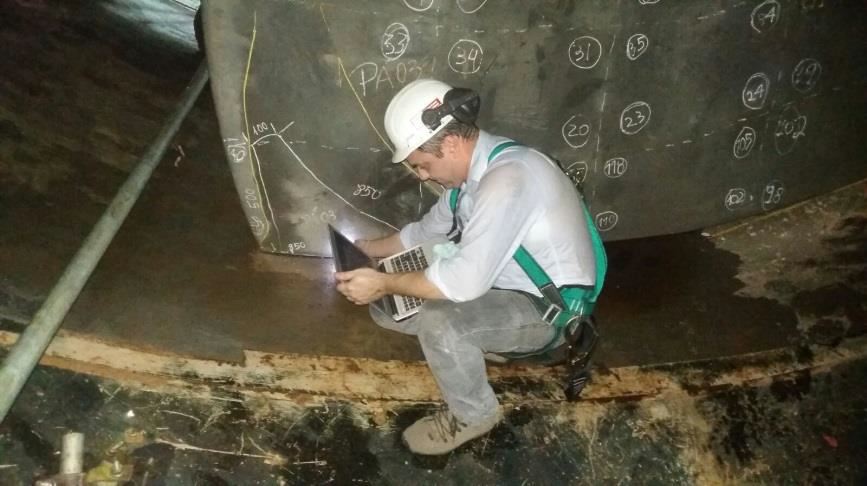
\includegraphics[width=0.9\linewidth, height=4cm]{figs/manolo} 
\caption{A equipe técnica analisa a pá verificando o desgaste do coating
existente e se existem danos a pá em si.}
\label{fig:subim1}
\end{figure}

\begin{figure}[H] 
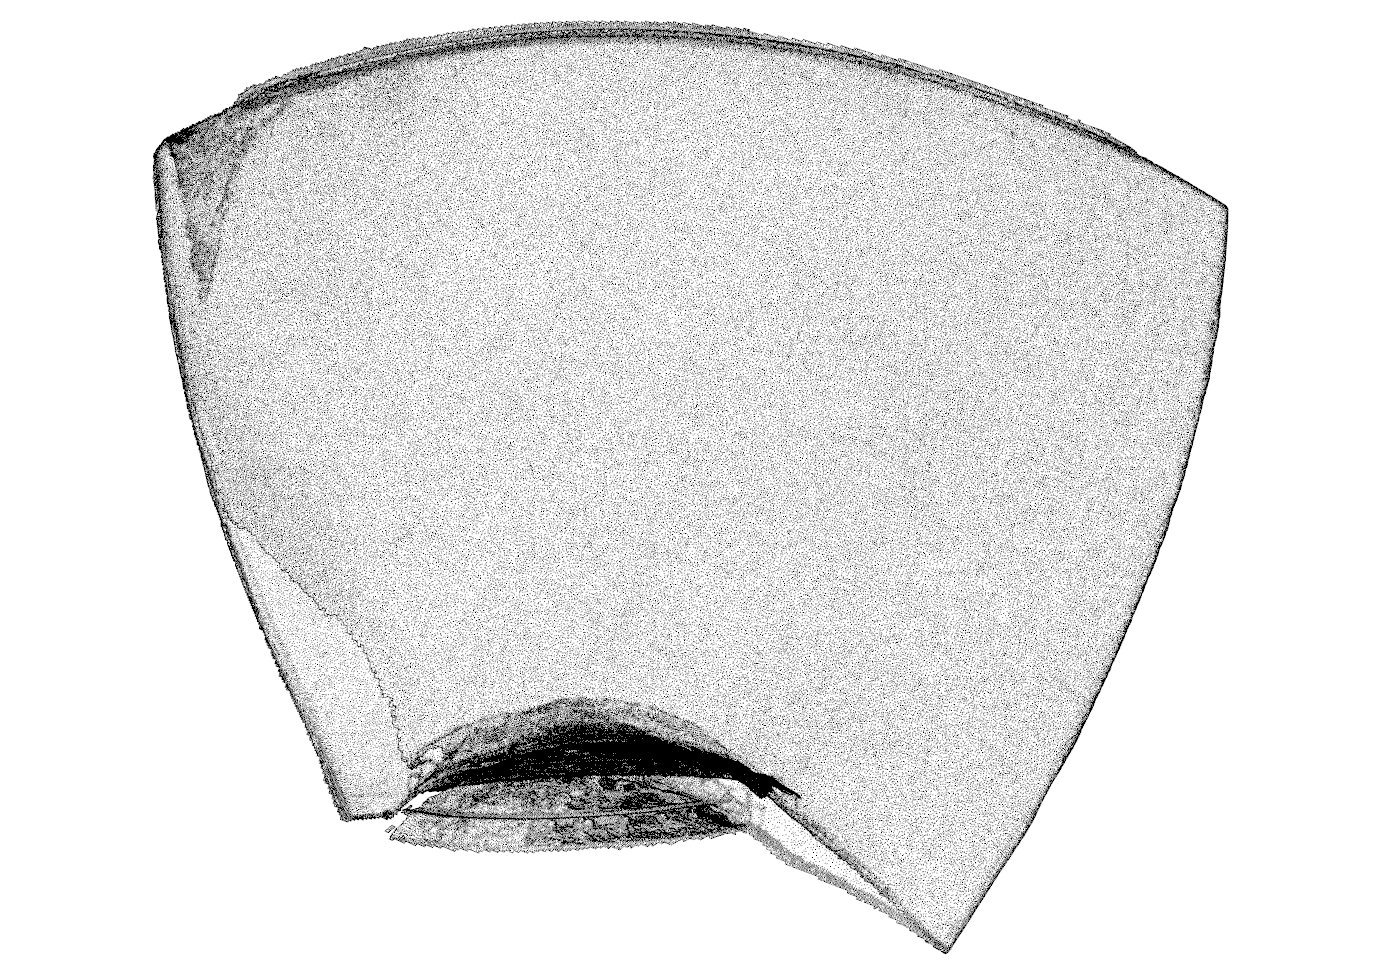
\includegraphics[width=0.9\linewidth, height=4cm]{figs/modelo_pa_faro}
\caption{Dado a necessidade de reparo um laser scanner de metrologia é
utilizado para mapear o dano com uma precisão de 2mm.}
\end{figure}

\begin{figure}[H]
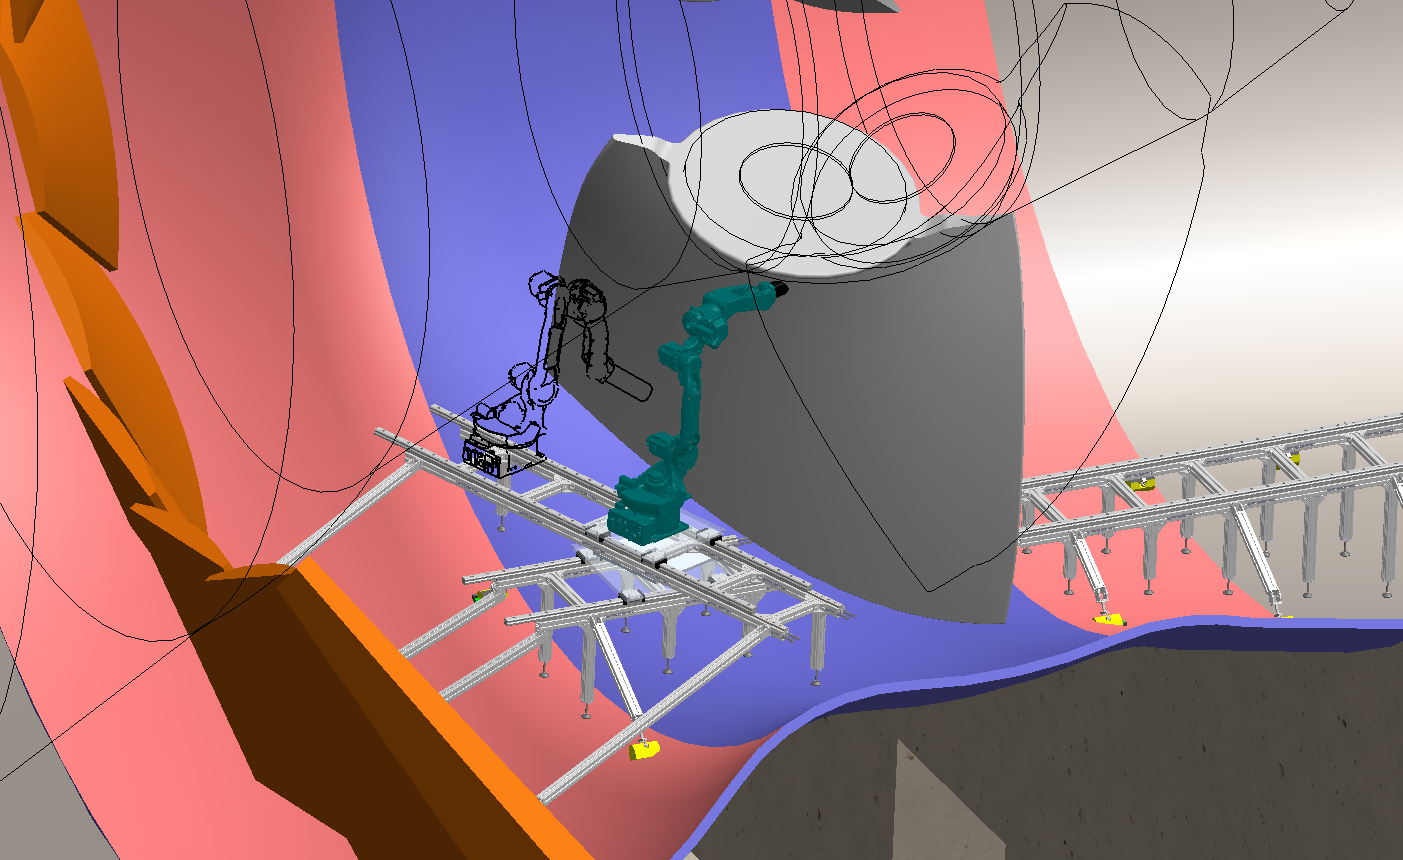
\includegraphics[width=0.9\linewidth, height=4cm]{figs/EMMA_Base_Secundaria_01} 
\caption{Um trilho modular é instalado no ambiente e aconrado através de pinos
magnéticos. O trilho é utilizado para levar o manipulador até a pá e movimentar
o manipulador ao longo da área de trabalho.}
\end{figure}

\begin{figure}[H]
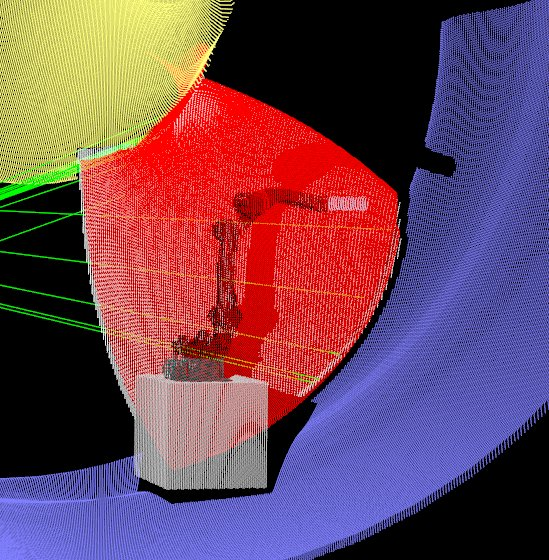
\includegraphics[width=0.9\linewidth, height=4cm]{figs/localizacao}
\caption{Algoritmo de processamento de nuvens de pontos analisam um scan laser
do ambiente e estimam a posição relativa entre o manipulador e a pá.}
\end{figure}


% \begin{figure}[H] 
% \begin{subfigure}{0.5\textwidth}
% 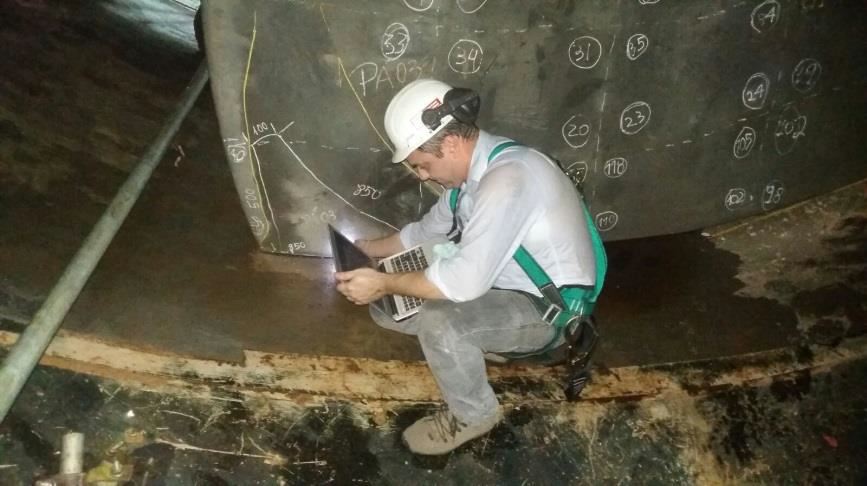
\includegraphics[width=0.9\linewidth, height=4cm]{figs/manolo} 
% \caption{A equipe técnica analisa a pá verificando o desgaste do coating
% existente e se existem danos a pá em si.}
% \label{fig:subim1}
% \end{subfigure}
% ~
% \begin{subfigure}{0.5\textwidth}
% \label{fig:subim2}
% 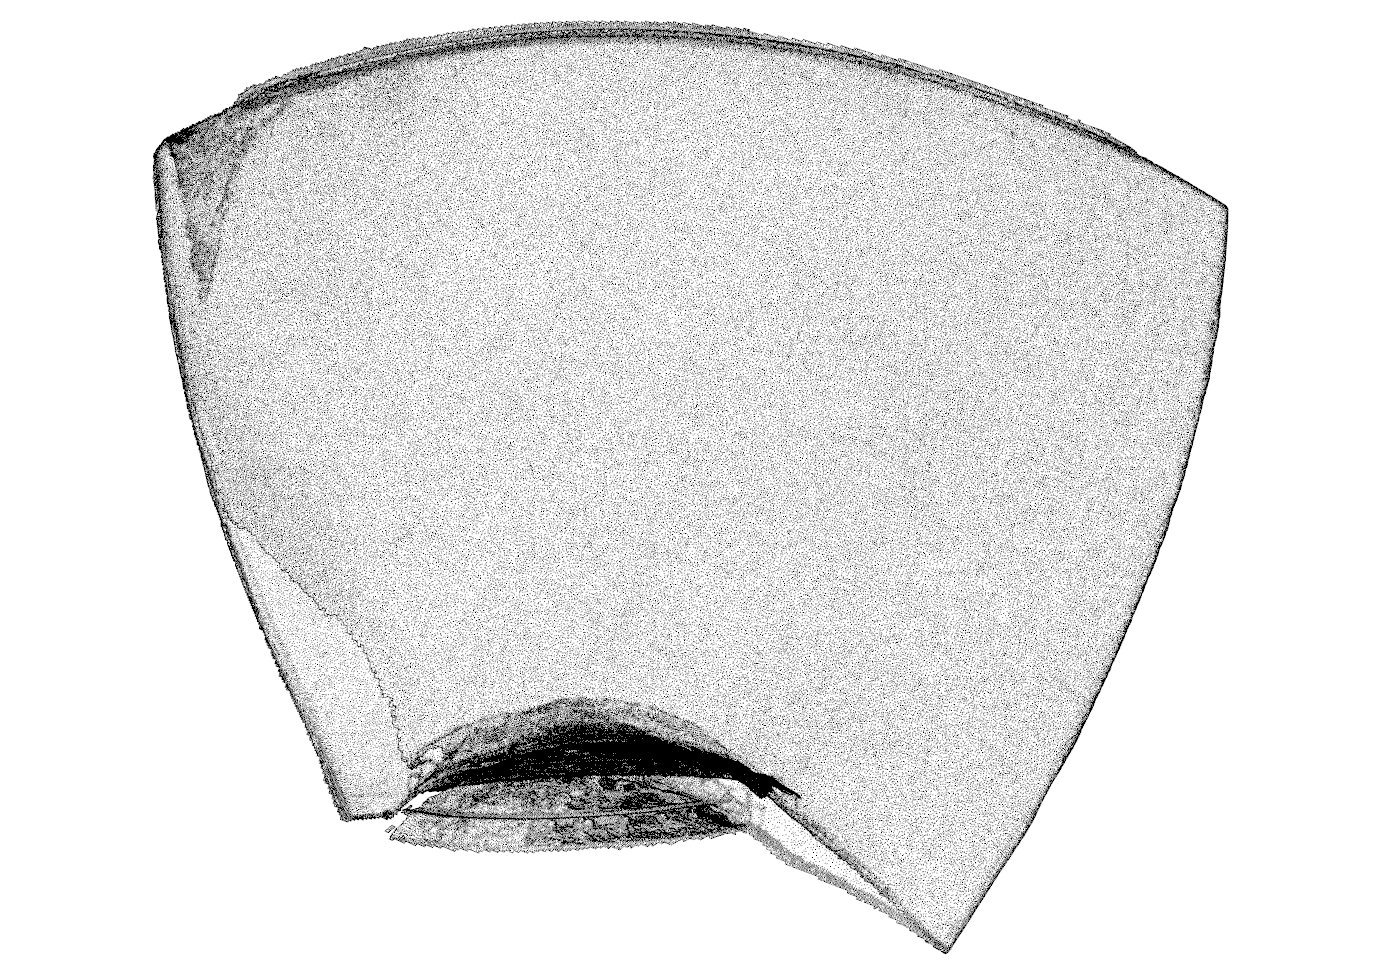
\includegraphics[width=0.9\linewidth, height=4cm]{figs/modelo_pa_faro}
% \caption{Dado a necessidade de reparo um laser scanner de metrologia é
% utilizado para mapear o dano com uma precisão de 2mm.}
% \end{subfigure}
%  \label{fig:image2}
% \end{figure}
% 
% \begin{figure}[H]
% \ContinuedFloat
% \begin{subfigure}{0.5\linewidth}
% 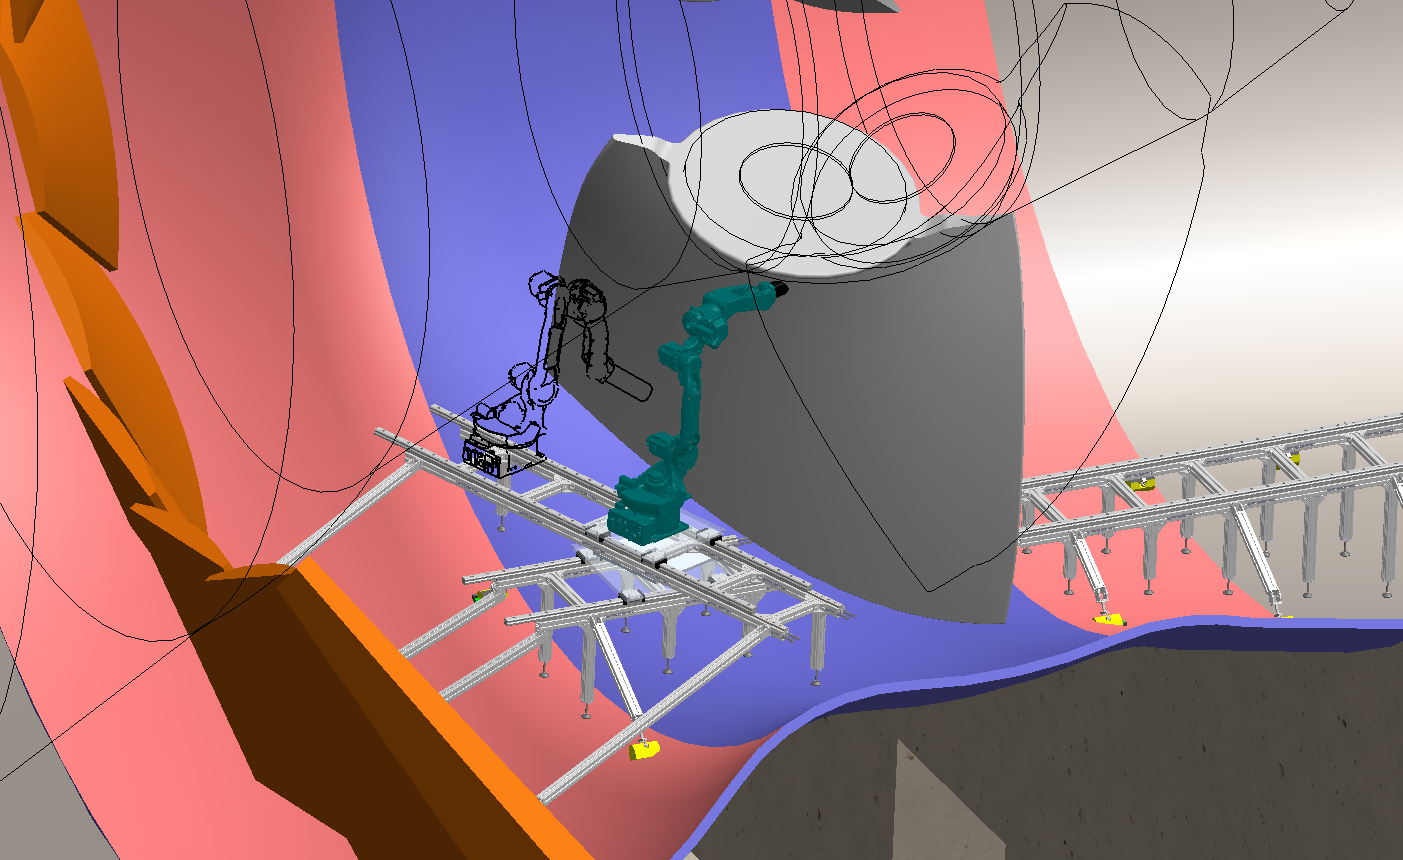
\includegraphics[width=0.9\linewidth, height=4cm]{figs/EMMA_Base_Secundaria_01} 
% \caption{Um trilho modular é instalado no ambiente e aconrado através de pinos
% magnéticos. O trilho é utilizado para levar o manipulador até a pá e movimentar
% o manipulador ao longo da área de trabalho.}
% \end{subfigure}
% ~
% \begin{subfigure}{0.5\linewidth}
% \label{fig:subim2}
% 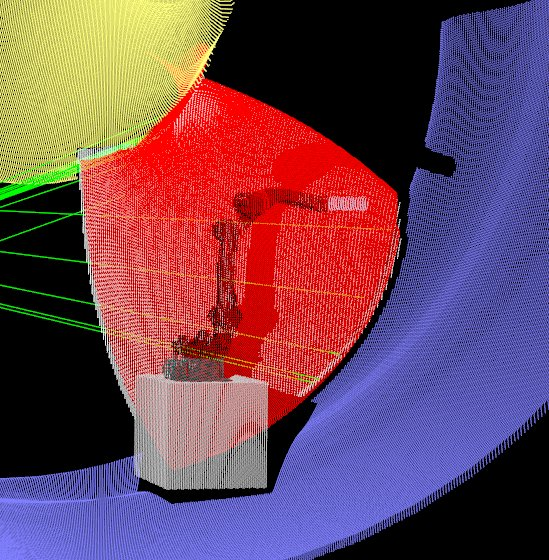
\includegraphics[width=0.9\linewidth, height=4cm]{figs/localizacao}
% \caption{Algoritmo de processamento de nuvens de pontos analisam um scan laser
% do ambiente e estimam a posição relativa entre o manipulador e a pá.}
% \end{subfigure}
%  \label{fig:image2}
% \end{figure}



% \begin{figure}[h!]
% \centering
% \captionsetup[subfigure]{position=b}
% \caption{3D printed wax mould post processing}
% \label{fig:Mould}
% \subcaptionbox{Um trilho modular é instalado no ambiente e aconrado através de pinos
% magnéticos. O trilho é utilizado para levar o manipulador até a pá e movimentar
% o manipulador ao longo da área de
% trabalho.\label{fig:MouldWithSupport}}{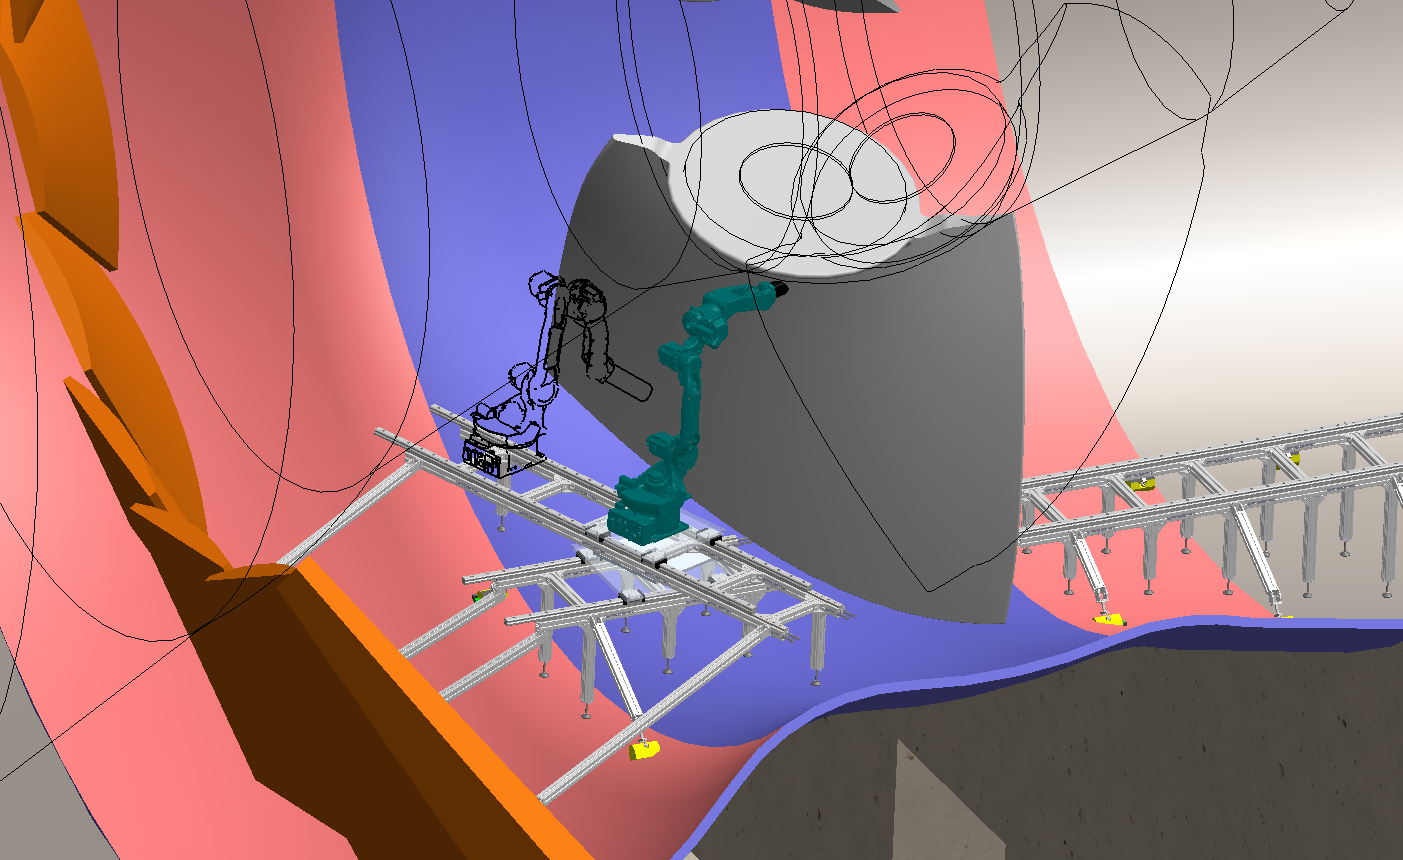
\includegraphics[width=0.5\linewidth, height=4cm]{figs/EMMA_Base_Secundaria_01}}
% \subcaptionbox{Algoritmo de processamento de nuvens de pontos analisam um scan laser
% do ambiente e estimam a posição relativa entre o manipulador e a pá.
% \label{fig:MouldAfterWashing}}{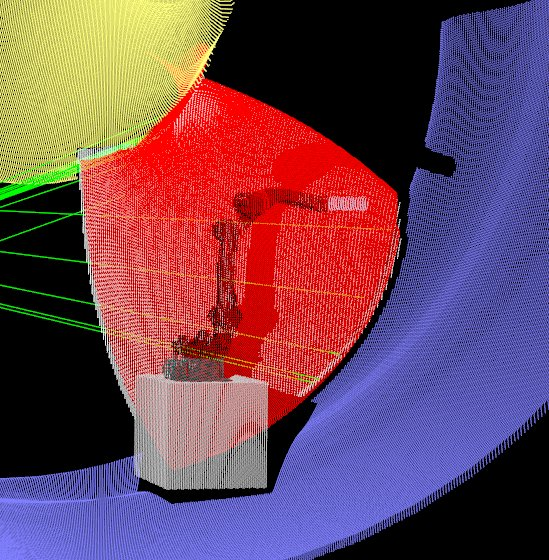
\includegraphics[width=0.5\linewidth, height=4cm]{figs/localizacao}}
% \end{figure}
% \end{document}









\begin{figure}[H]
\ContinuedFloat
\begin{subfigure}{0.5\textwidth}
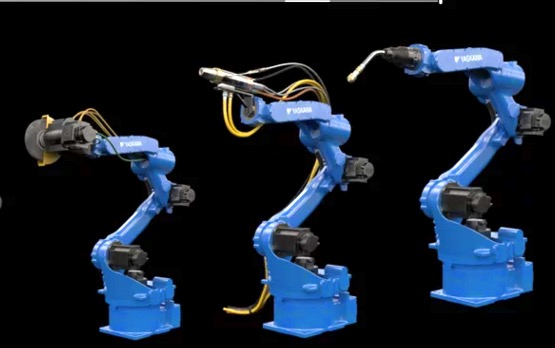
\includegraphics[width=0.9\linewidth, height=4cm]{figs/robots_evo} 
\caption{O equipamento necessário para a tarefa, seja soldagem, esmerilhamento
ou coating é instalado no manipulador e o ambiente e superfície são preparados.}
\end{subfigure}
~
\begin{subfigure}{0.5\textwidth}
\label{fig:subim2}
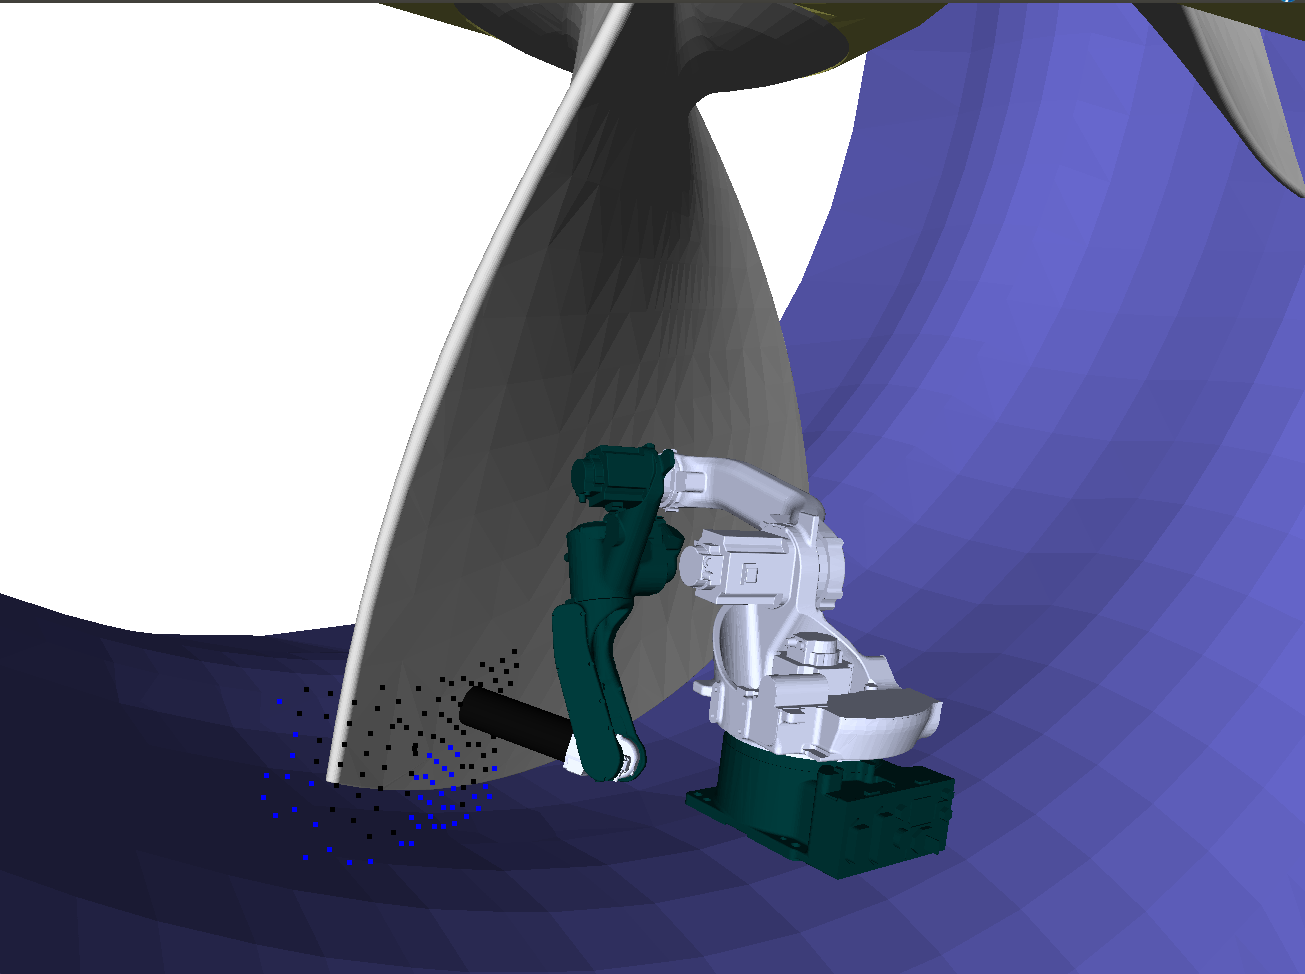
\includegraphics[width=0.9\linewidth, height=4cm]{figs/footleft}
\caption{O algoritmo estima e executa a trajetória para a tarefa planejada.}
\end{subfigure}
 \label{fig:image2}
\end{figure}

O resultado do processo é uma pá restaurada e protegida, aumentando a eficiência
de geração e vida útil da mesma. 

\section{Motivação}

Desgastes por corrosão, erosão e abrasão em pás de turbinas de hidroelétricas
resultam em perda do perfil hidráulico, reduzindo assim a eficiência de geração.
O desgaste reduz também a vida útil da turbina, o tempo de operação entre
paradas de manutenção, assim como, aumentam os custos de manutenção e o tempo
necessário de parada de máquina para a realização do reparo. Logo, significa uma
perda da eficiência de geração, e por consequente um impacto econômico
significativo na operação.
A aplicação de revestimento aumenta a resistência do material contra os
desgastes, custando em torno de 20\% do valor de uma peca nova e representando
um aumento da vida útil em mais de 300\%. Entretanto, dados as limitações da
tecnologia atual, só é possível aplicar o revestimento em bancada, logo, antes
da instalação das pás. Logo, o desenvolvimento tecnológico que possibilite
reaplicar a camada de revestimento dentro do circuito hidráulico resultaria em
um ganho significativo na geração e redução dos custos de operação.
Antes de aplicar o revestimento é necessário reparar a pá recuperando o perfil
hidráulico da mesma, quanto maior a precisão da recuperação do perfil hidráulico
maior a eficiência de geração. Logo, a robótica se torna a ferramenta ideal para a tarefa.

\section{Objetivo}

O objetivo geral do projeto é desenvolver e testar uma metodologia que permita
utilizar a robótica para reparar e revestir pás instaladas em circuitos hidráulicos.

Os objetivos específicos são determinar as metodologias: 

\begin{itemize}
  \item definir o manipulador ótimo para cada hidroelétrica 
  \item movimentar o manipulador dentro do circuito hidráulico
  \item estimar a posição do manipulador com relação ao meio
  \item material e técnica de coating e reparo 
  \item preparar o meio e superfície
  \item logística para instalar um sistema robótico no circuito hidráulico
  \item determinar os riscos associados
  \item planejar e executar a manipulação
  \item representar as diferentes informações do processo para um operador
  \item verificar as perdas de carga do processo de revestimento
  \item integrar e utilizar as diversas ferramentas
  \item mapear o perfil hidráulico e medir os danos
\end{itemize}

\section{Originalidade}

Não existe nenhuma solução ou estudo realizado sobre a aplicação de revestimento
dentro do circuito hidráulico sem desinstalar as pás da turbina. A aplicação de
revestimento para proteção contra abrasão, cavitação, corrosão e erosão em peças
de turbinas de hidrelétricas realizado atualmente é limitada a trabalho em
bancada com a peça desinstalada. O desafio de realizar o trabalho de
revestimento dentro do circuito hidráulico se dá pela dimensão da escotilha de
acesso, que limita o tamanho do robô, pelo posicionamento do robô com relação a
pá da turbina, que se encontra a alguns metros do solo, pelo processo de
aplicação que requer velocidade constante utilizando uma pistola pesada e pelo
controle de temperatura e humidade necessários. Esta pesquisa é inovadora no
setor elétrico brasileiro e é um avanço com relação ao estado da arte.

\section{Aplicabilidade}

A metodologia desenvolvida no projeto  poderá ser aplicada na maioria das
hidroelétricas de médio ou grande porte. A metodologia determina o tamanho e
modelo de manipulador ótimo para o circuito hidráulico em questão, assim como,
qual material de coating a ser aplicado. A restrição para aplicação da tecnologia é
apenas dada pelo espaço entre as pás, em hidroelétricas de pequeno porte a arma
de coating não cabe entre as pás. Logo, a abrangência é nacional, entretanto com
restrição de uso em pequenas unidades geradoras.

\section{Relevância}

A matriz geradora Brasileira é constituída em sua maioria por geração
hidráulica, com um grande número de centrais em rios tipos corredeiras que
possuem reservatórios pequenos. Neste tipo de rio não há tempo de sedimentação
das partículas sólidas na água, essas partículas sólidas, mesmo em quantidades
pequenas, geram um elevado nível de desgaste por erosão e cavitação. Logo, o
projeto é de relevância para o setor elétrico e para a nação, pois aumenta a
eficiência da matriz energética Brasileira, aumenta a disponibilidade da máquina
para geração e reduz os custos de manutenção, representando uma melhora
econômica e social.

\section{Capacitação}

A pesquisa e o desenvolvimento (P\&D) tem como propósito fomentar o avanço
tecnológico e novas maneiras de desenvolver um tipos específicos de conhecimento
no país. O desenvolvimento do EMMA, no âmbito P\&D é um exemplo de como a
parceria entre agências do governo, empresa e universidades podem colaborar para
a capacitação tecnológica e o desenvolvimento de novas tecnologias.

O projeto EMMA possui 4 pesquisadores inscritos no mestrado. Os temas são todos
a pesquisa no campo da robótica, sendo a previsão de conclusão das teses
esperada para a fase 2 e fase 3 do EMMA. Os alunos de mestrado e seus
respectivos cursos são:

\begin{itemize}
  \item Estevão Fróes Ferrão, Programa de Engenharia Mecânica/COPPE, Rio de
  Janeiro
  \item Gabriel Alcantara Costa Silva, Programa de Engenharia Elétrica/COPPE,
  Rio de Janeiro
  \item Eduardo Elael de Melo Soares, Programa de Engenharia Elétrica/COPPE, Rio
  de Janeiro
  \item Julia Ramos Campana, Departamento de Artes e Design, PUC, Rio de Janeiro
\end{itemize}

Para o comprimento dos requisitos de segurança do Ministério do Trabalho e
Emprego, a equipe do projeto foi submetida à capacitação em segurança, nas
normas relevantes às situações encontradas no interior do circuito hidráulico. As certificações foram nas
seguintes normas:

\begin{itemize}
  \item NR10 - Segurança e Instalações e Serviços em Eletricidade
  \item NR33 - Segurança e Saúde nos Trabalhos em Espaços Confinados
  \item NR35 - Trabalho em Altura
\end{itemize}

Os seguintes pesquisadores foram capacitados no curso:

\begin{itemize}
  \item Estevão Fróes Ferrão, Programa de Engenharia Mecânica/COPPE
  \item Gabriel Alcantara Costa Silva, Programa de Engenharia Elétrica/COPPE
  \item Renan Sales de Freitas, Programa de Engenharia Elétrica/COPPE
  \item Eduardo Elael de Melo Soares, Programa de Engenharia Elétrica/COPPE
  \item Julia Ramos Campana %TODO Julia departamento
\end{itemize}
A pesquisa no projeto EMMA proporcionou a elaboração de dois artigos
submetidos/publicados em revistas, abordando os seguintes tópicos: 

\begin{itemize}
  \item Estado da arte e design conceitual de soluções robóticas para
  revestimento de turbinas hidráulicas \textit{in situ} (State of the art and
  conceptual design of robotic solutions for \textit{in situ} hard coating of
  hydraulic turbines).
  \item Solução Conceitual e estudo de viabilidade técnica para para
  revestimento de turbinas hidráulicas \textit{in situ} (EMMA - A robotic
  system for \textit{in situ} hydropower turbine hard coating).
\end{itemize}

\section{Razoabilidade dos Custos}

Atualmente, após a instalação da unidade geradora, não existe método disponível
para proteger a ogiva geradora contra os desgastes de sua utilização. Sendo,
infelizmente, a recuperação sempre o caminho e isso pode ser estimado entre 90 e
120 dias de UG parada. A frequência de paradas de recuperação variam dependendo
da idade da unidade geradora, material, tipo de bacia e etc. A única certeza é
que um dia será necessário. A aplicação de revestimento pode ser realizada
durante as paradas planejadas, sem perda de tempo de geração.
De acordo com a tabela de situação de cavitação em turbina hidráulica no Brasil
(Out/97), em média 5 unidades geradoras apresentaram  cavitação a cada 24.071
horas de operação (2,7 anos), das 36 instalações analisadas. Logo, em Jirau a
aplicação do revestimento in situ significaria em um aumento da disponibilidade
de geração de 600 dias a cada 2,7 anos, considerando turbinas de 75 MW de
potencia, seria equivalente a 1.080.000 MW a cada 2,7 anos.

\section{Metodologia adotada}

O projeto EMMA foi dividido em 3 fases, sendo cada fase um projeto distinto.
Cada fase avançando a tecnologia ao longo da cadeia de inovação. Na primeira
fase foi desenvolvido a metodologia/conceito. Na segunda fase será feito o
desenvolvimento experimental testando o sistema de coating. Na terceira fase
será expando a solução para incluir reparo e validar a tecnologia em outras
centrais hidroelétricas.

Ao início da primeira fase não se sabia se existiria uma solução para o
problema. Os requisitos de acesso, operação e coating são extremamente
limitantes. A metodologia adotada na fase 1 para desenvolver o conceito da
solução foi:

\textbf{Etapa 1}: Levantamento dos requisitos do ambiente, tarefas e
procedimentos.
Estudo do estado da arte e bibliografias existente no tópico. Baseado nos
requisito e estado da arte foi definido uma solução conceito que atende ao problema.

\textbf{Etapa 2}: A solução conceito foi detalhada. Neste detalhamento foi
determinando os equipamentos e fornecedores que seriam adequados a serem
utilizados na solução. Assim como foi realizado pesquisa bibliográfica para
determinar quais os algoritmos e técnicas mais adequadas a serem implementadas
como parte da solução.

\textbf{Etapa 3}:  A solução conceito detalhada foi validada através de
simulações e experimentos em laboratório de alguns conceitos chaves. Um exemplo
foi utilizar o openrave para simular o processo de movimento do manipulador e
experimentos de campos da fixação por pino magnético.

\section{Estratégia de difusão}

A estratégia de difusão adotada no projeto foi a realização de um evento de
transferência de conhecimento dentro da faculdade de porto velho que inclui não
apenas os funcionários da ESBR, mas também os alunos e professores da faculdade.
O evento serviu como um “aulão” em pesquisa aplicada em robótica. Onde cada
pesquisador do projeto, em sua maioria alunos de mestrado da UFRJ, deram uma
aula sobre seus tópicos de pesquisa dentro do projeto.

%TODO foto do evento

\section{Melhorias de processo, equipamento e sistema}

O projeto representa uma melhoria no processo de reparo das pás de turbina
hidroelétricas que atualmente são feitas manualmente. Espera-se que o processo
robótico consiga recuperar o perfil hidráulico para uma margem de 2-5 mm do perfil original.

O fato de o EMMA também realizar o revestimento das turbinas instaladas, algo
antes impossível, o projeto representa uma melhoria no equipamento (pás das
turbinas), pois as mesmas se tornam mais resistentes aos danos corrosão, erosão e abrasão.

Por fim, o projeto também representa uma melhoria a todo sistema de geração de
energia elétrica. Pois, aumenta a vida útil das turbina e mantêm o perfil
hidráulico original, logo um impacto direto no aumento da geração.

\section{Pesquisa Correlatas}

\textbf{Google Schoolar, IEEE, Field Robotics, ... }: nenhum resultado foi
encontrado na revisão bibliográfica para uma solução robótica de aplicação de
revestimento em turbinas hidroelétrica já instaladas no Brasil e no exterior. A
pesquisa revela apenas o desenvolvimento de robôs para reparos in situ da
turbina, capazes de realizar soldagem, em exemplo RoboTurb da UFSC e Scompi da
Hydro-Quebec. Ambos não aplicáveis ao problema de revestimento devido as
limitações do manipulador robótico nos sistemas.

\textbf{INPI}: Nenhuma patente foi encontrada que se enquadre como o produto
objeto da pesquisa e desenvolvimento aqui proposta.

\textbf{ANEEL}: nenhum resultado foi encontrado na base de dados da ANEEL
relevante a um robô para revestimento. Os resultados encontrados referiam-se a
um Robo que inspeciona e corrige problemas em linhas de transmissão; Sistema
Multi-robôs Aéreos para Inspeção de Linhas e Robô para Inspeção Visualde
caldeiras.

\section{Instituição e Equipe}

O LEAD (Laboratório de Controle e Automação, Engenharia de Aplicação e
Desenvolvimento) é fruto de uma parceria entre a Petrobras e a Universidade
Federal do Rio de Janeiro (UFRJ) que visa ao desenvolvimento de novas
tecnologias na área de Automação e Controle.
Na avaliação da estatal brasileira de petróleo, ‘‘o laboratório reforça a
estratégia de desenvolvimento em conjunto de novas tecnologias, o que traz
benefícios tanto para as universidades, que realizam suas pesquisas acadêmicas
em laboratórios de ponta, quanto para a Petrobras que, ao compartilhar
conhecimentos, cria competências para superar seus desafios tecnológicos e
empresariais”.

DARLAN PARAGRAFO RIJEZA

%TODO DARLAN PARAGRAFO RIJEZA

A equipe técnica alocada para a realização do projeto EMMA:

\begin{itemize}
  \item Renan Salles de Freitas, Engenheiro de Controle e
Automação pela UFRJ, Rio de Janeiro, Brasil, e Candidato a Mestre em Ciências em Engenharia Elétrica
pelo Programa de Engenharia Elétrica, COPPE/UFRJ, Rio de Janeiro, Brasil. No
projeto EMMA, Renan é membro da equipe de Controle e Robótica, e responsável
pelas seguintes atividades: Manipuladores industriais: pesquisa de
mercado, análise cinemática, dinâmica e controle; Desenvolvimento do ambiente de
simulação para análise de soluções; Análise de viabilidade técnica do EMMA pela
visão da robótica e do controle; Desenvolvimento e simulação de algoritmos de
planejamento de trajetória.

  \item Estevão Fróes Ferrão possui graduação em Engenharia Mecânica pela Universidade
Federal do Rio de Janeiro (UFRJ), atualmente cursando o mestrado no Programa de Engenharia
Mecânica (PEM-COPPE/UFRJ). Faz parte da equipe do Projeto EMMA, como
Pesquisador/Engenheiro contratado pelo LEAD. Atua na área de Projeto Mecânico,
sendo resposável pela pesquisa, projeto e desenvolvimento de uma solução
mecânica para uma base com graus de liberdade que permitem o posicionamento do
robô utilizado.

\item Julia Ramos Campana é formada em Comunição Técnica e Mídia pelo Instituto de
Tecnologia e Illinois, pós graduada em Design Digital pela Vancouver Film School
e em Gerenciamento de Projeto pela Universidade da Columbia Britânica, é
atualmente aluna do Mestrado em Design pela PUC-RJ. Julia exerce a função de
Designer de interface e Usabilidade no projeto EMMA, trabalhando no
desenvolvimento do software de controle do sistema EMMA e em todas as questões
relacionadas aos usuários, testes e interações humano-automação da pesquisa.
\item Eduardo Elael de Melo Soares, Engenheiro de Controle e Automação pela UFRJ, Rio
de Janeiro, Brasil, e mestrando em Ciências em Engenharia Elétrica pelo
Programa de Engenharia Elétrica, COPPE/UFRJ, Rio de Janeiro, Brasil. No projeto
EMMA, Eduardo é membro da equipe de Controle e Robótica, e responsável pelas
seguintes atividades: Manipuladores de pequeno porte: Pesquisa e análise
geométrica; Realimentação de segurança: Pesquisa de laser 1D para uso em tempo
real; Reconhecimento de ambiente: Escolha e adaptação de técnicas para
reconhecimento da posição do Robô no ambiente; Desenvolvimento e simulação de
algoritmos de planejamento de trajetória.
\item Gabriel Alcantara Costa Silva, Engenheiro de Controle e Automação pela
UFRJ, Rio de Janeiro, Brasil, e mestrando em Ciências em Engenharia Elétrica pelo
Programa de Engenharia Elétrica, COPPE/UFRJ, Rio de Janeiro, Brasil. No projeto
EMMA, Eduardo é membro da equipe de desenvolvimento de software para sistemas
robóticos, e responsável pelas seguintes atividades: Desenvolvimento de técnicas
em visualização, localização e mapeamento 3D; Identificação e
Localização de objetos; Integração do sistema.

\end{itemize}








    
    
  


\chapter{Plano de Projeto}\label{chap::planejamento}


\section{Etapa 1 - Fundação Coppetec}

\begin{figure}[H]
\centering
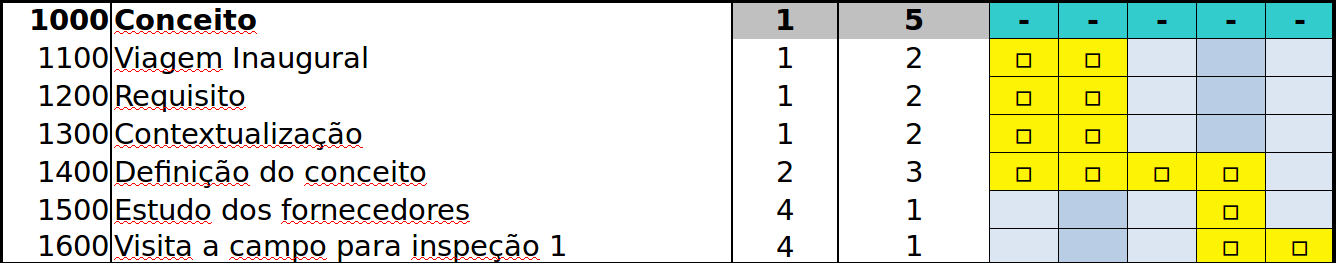
\includegraphics[width=0.9\columnwidth]{figs/etapa1_completo}
\end{figure} 

\textbf{1000 Conceito:} A etapa 1000 do projeto foi executada como prevista. O
objetivo da etapa foi a determinação dos requisitos do problema e concepção de
possíveis soluções. As seguintes trabalhos foram executados dentro desta etapa

\noindent
\textbf{1100 Viagem Inaugural:} Assinatura do termo inaugural do projeto e
análise em campo da problemática

Etapa executada como previsto. 

\begin{figure}[H]
\centering
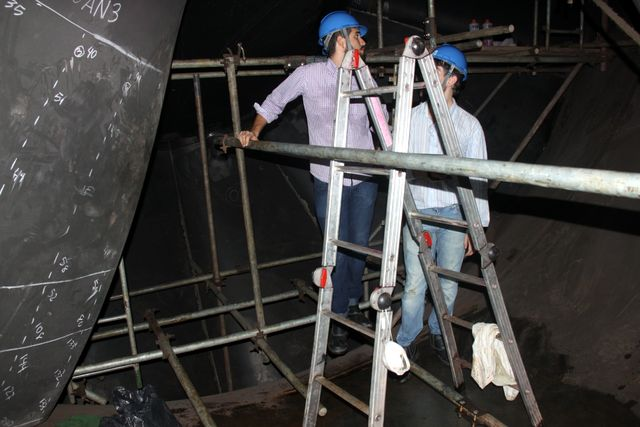
\includegraphics[width=0.6\columnwidth]{figs/img_4967}
\caption{Pesquisadores analisando o ambiente.}
\end{figure}

\noindent
\textbf{1200 Requisito:} Fazer levantamento dos requisitos que afetam a
instalação e utilização de um robô dentro circuito hidráulico.

Etapa executada como previsto. Foram levantados todos os requisitos de acesso,
ambiente e processo de coating.

\noindent
\textbf{1300 Contextualização:} Levantamento das tecnologias existentes no para
aplicações de revestimento em ambientes confinados.

Etapa executada como previsto. Diversas tecnologias foram pesquisadas, como o
robô scompi da hidroquebec. Nenhuma das soluções atuais atendiam os requisitos
de operação do projeto.

\noindent
\textbf{1400 Definição dos conceitos:} Definição de uma solução de um robô capaz
de operar no ambiente e realizar tarefas de revestimento.

Etapa executada como previsto. Foram levantados 3 conceitos viáveis, os quais
foram analisados chegando ao conceito proposto dentro do projeto. Utilizar um
manipulador industrial, acessando o circuito hidráulico pela escotilha de
acesso, com movimentação através de trilhos modulares e alinhamento, mapeamento
e planejamento de trajetória baseado em scan 3D a laser do ambiente.

\begin{figure}
\centering
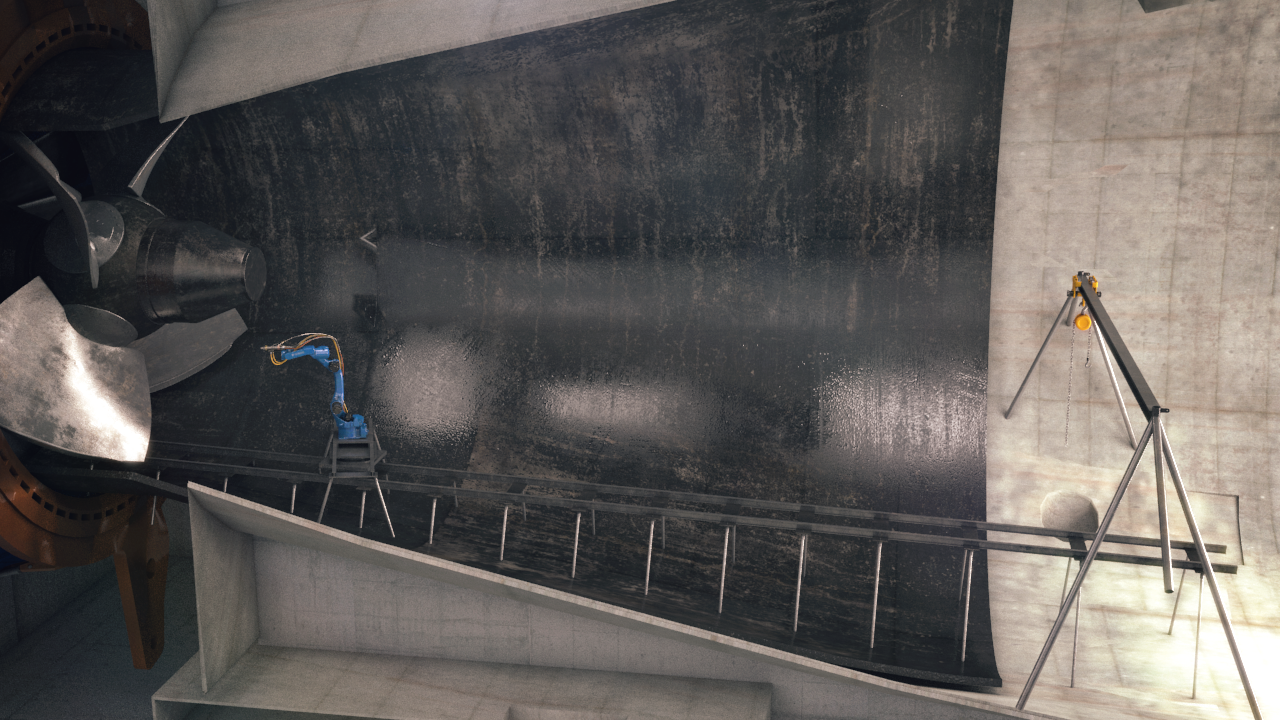
\includegraphics[width=0.9\columnwidth]{figs/turbine_evo}
\caption{Solução conceito.}
\end{figure}

\noindent
\textbf{1500 Estudo dos fornecedores:} Definição dos fornecedores do equipamento
necessário para a pesquisa

Etapa executada como previsto. Foram analisados mais de 50 modelos de
manipuladores distintos, sendo que 5 atendiam os requisitos do problema como
possíveis soluções.

\begin{figure}[h!]
\centering
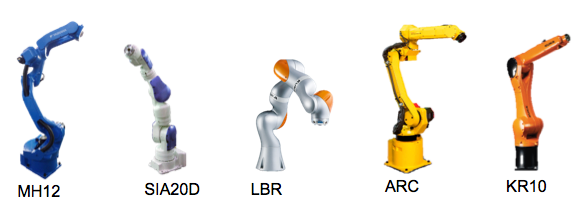
\includegraphics[width=0.9\columnwidth]{figs/robots}
\caption{Possíveis modelos de manipuladores que atendem os requisitos.}
\end{figure}

\noindent
\textbf{1600 Visita a campo para inspeção 1:} foi realizada uma visita inicial
a campo para juntamente com revisão bibliográfica sobre o tema “desgaste”
coletar dados de campo através de inspeção nas pás das turbinas. Essas inspeções
foram realizadas ao longo do projeto para confrontar com o que existe na
bibliografia.


\section{Etapa 02}

\begin{figure}[H]
\centering
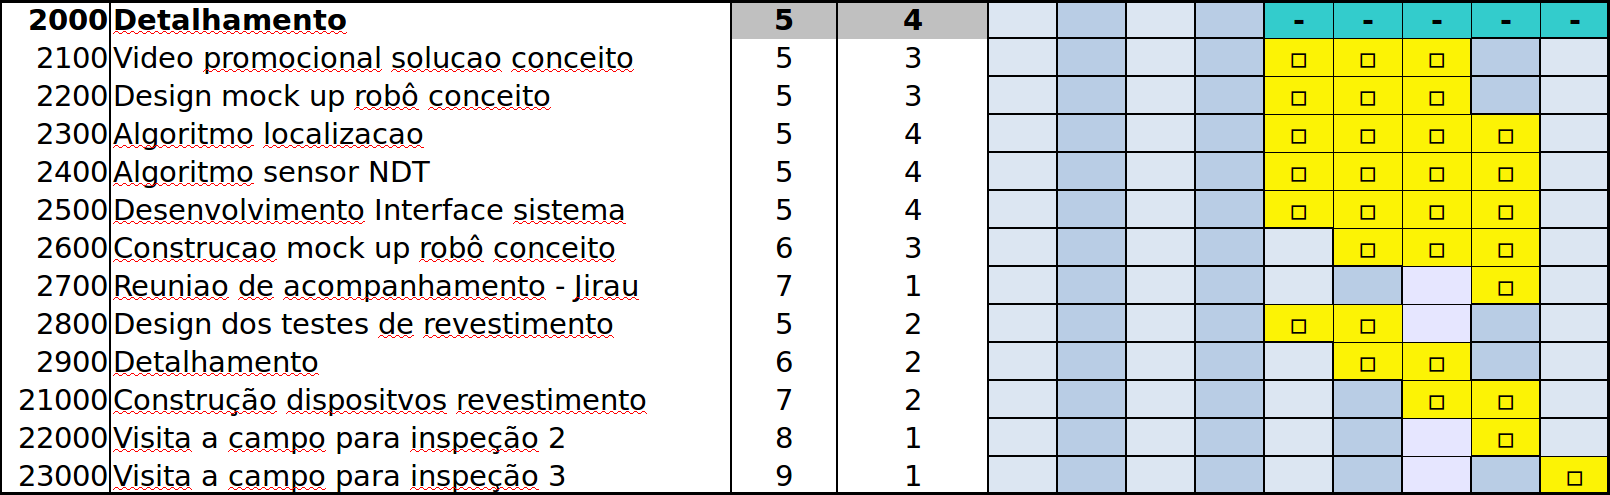
\includegraphics[width=0.9\columnwidth]{figs/etapa2_completo}
\end{figure} 

\noindent
\textbf{2000 Detalhamento:} A etapa 2000 do projeto foi executada existindo
variações entre previsto e executado. O objetivo da etapa foi a análise das
proposições mediante estudos teóricos e design detalhado da possível solução e sistema

\noindent
\textbf{2100 Video promocional solução conceito:} Animação 3D da solução
conceito

Houve atraso no processo de contratação e aprovação do script. A tarefa foi
executada com 3 meses de atraso. Entretanto, o mesmo não impactou no projeto,
pois não era uma tarefa de pré-requisito.

\noindent
\textbf{2200 Design mock up robô conceito:} Design em CAD / Solidworks do
conceito do robô

Tarefa executada como prevista. Foram realizado diversos designs para possíveis
bases para a solução conceito, assim como análises geométricas, cinemática,
dinâmica e de manipulabilidade para definir o manipulador.

\begin{figure}\centering
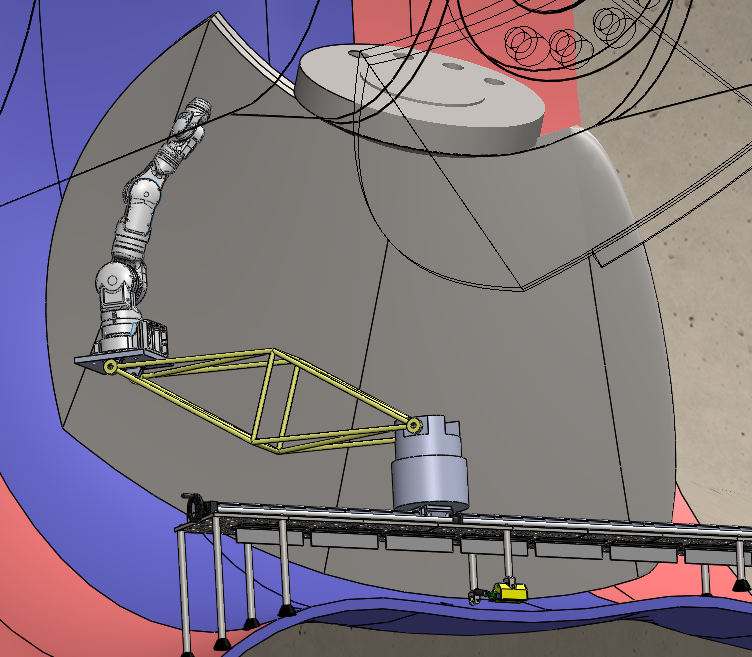
\includegraphics[width=0.6\columnwidth]{figs/EMMA_Base_Conceito_PRR}
\caption{Possível base para o manipulador dentro do ambiente do circuito
hidráulico.}
\end{figure} 


\noindent
\textbf{2300 Design dos testes de revestimento:} %TODO DARLAN

\noindent
\textbf{2400 Algoritmo de localização:} definir o algoritmo/técnica que irá
localizar o robô com relação a turbina.

Tarefa executada como prevista. Foi determinado que o melhor e mais preciso
método é escanear o robô e a pá com um laser de metrologia e a estimar posição
relativa das nuvens de pontos resultantes.

\begin{figure}[H]
\centering
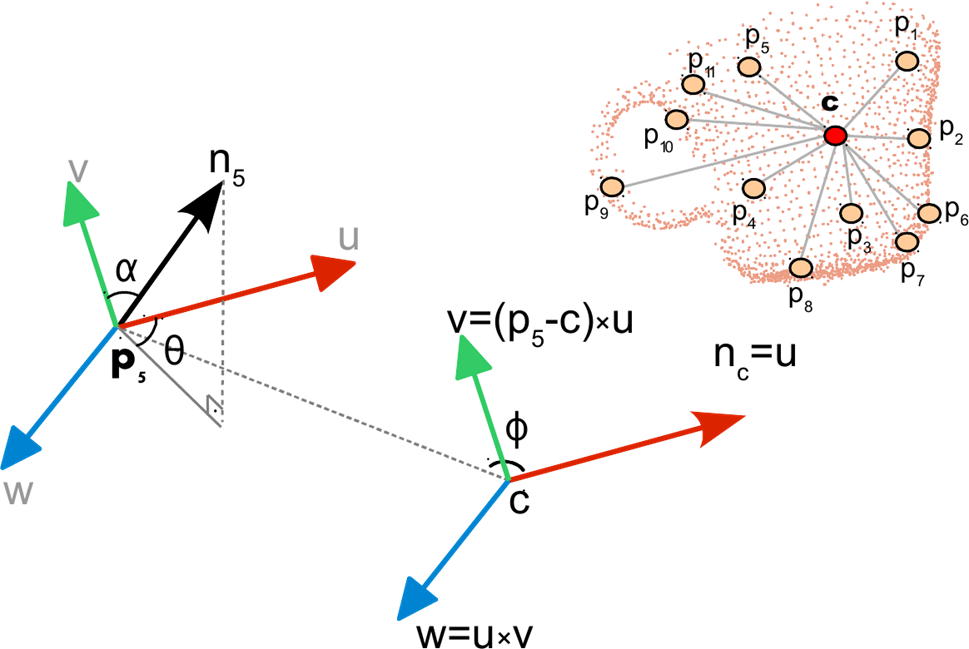
\includegraphics[width=0.6\columnwidth]{figs/pc_position}
\caption{Posição relativa entre duas nuvens de pontos.}
\end{figure} 

\noindent
\textbf{2500 Algoritmo sensor NDT:} Algoritmo que irá avaliar e mapear a
qualidade do revestimento.

Tarefa executada como prevista. Foi determinado que o método mais eficiente é
utilizar um humano para rapidamente realizar uma amostragem de alguns pontos com
sensor ultra-som manual. A solução robótica seria em uma alusão “matar um mosquito com basuca”.

\noindent
\textbf{2600 Desenvolvimento Interface sistema:} Interface gráfica de controle e
utilização do sistema

Essa tarefa foi estendida para 8 meses, se tornando uma teses de mestrado dada
sua complexidade. A solução conceito possui um volume muito grande de interação
e informação para o usuário. Logo, adotou-se um estudo metódico,
estabelecendo-se toda a metodologia para determinar a interface e como cada
informação será representada.

\noindent
\textbf{2700 Construção mock up robô conceito:} Construção do mock up do robô
que aplica o revestimento

Tarefa executada como previsto. Foi construído todo o ambiente do circuito
hidráulico e manipulador através de impressão 3D em uma escala 1:20.

\begin{figure}[h!]
\centering
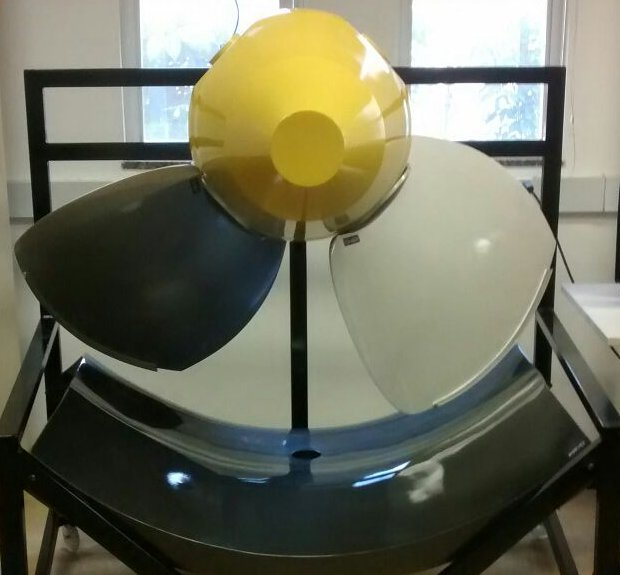
\includegraphics[width=0.6\columnwidth]{figs/maquete}
\caption{Maquete utilizada no desenvolvimento do conceito.}
\end{figure} 

  
\noindent
\textbf{2800 Design dos testes de revestimento:} %TODO DARLAN

\noindent
\textbf{2900 Reunião de acompanhamento:} Reunião de acompanhemento do projeto.
Tarefa executada como prevista.

\noindent
\textbf{21000 Construção dispositivos revestimento:}


\noindent
\textbf{22000 Visita a campo para inspeção 2:}


\noindent
\textbf{23000 Visita a campo para inspeção 3:}

\begin{figure}\centering
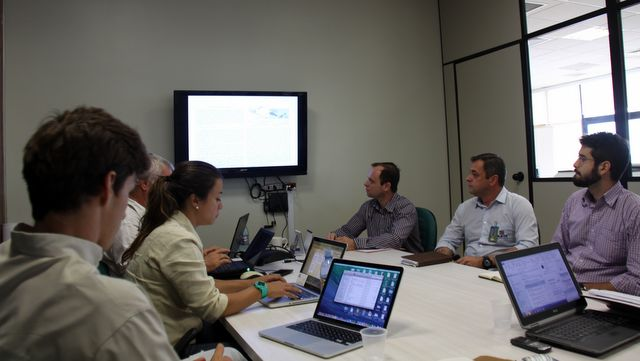
\includegraphics[width=0.6\columnwidth]{figs/img_4836}
\caption{Reunião de acompanhamento em Jirau.}
\end{figure} 

\section{Etapa 03} 

\begin{figure}[H]
\centering
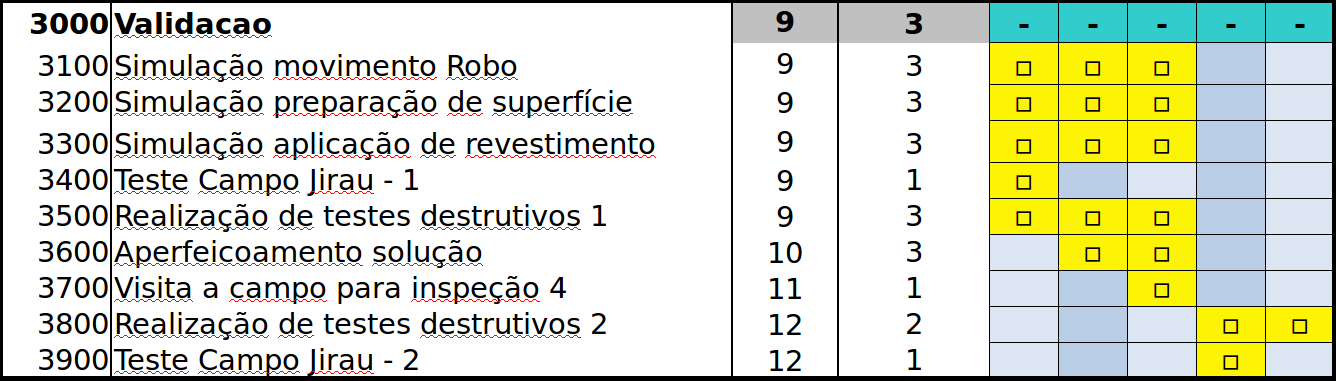
\includegraphics[width=0.9\columnwidth]{figs/etapa3_completo}
\end{figure} 

\noindent
\textbf{3000 Detalhamento:} A etapa 3000 do projeto foi executada existindo
variações entre previsto e executado. O objetivo da etapa é validação da solução
detalhada através de simulação e experimentos.

\noindent
\textbf{3100 Simulação movimento robô:} 
Simulação dos movimentos do robô sobre a turbina, verificando limites e singularidades

Tarefa executada como prevista. Foi utilizado o simulador Openrave.  

\noindent
\textbf{3200 Simulação preparação de superfície:}
Testes para avaliar a modificação do procedimento de jateamento para a sua adequação ao ambiente proposto no projeto;

\noindent
\textbf{3300 Simulação aplicação revestimento:}

Aplicação em amostras de testes para qualificação de materiais e procedimento de aspersão para posterior avaliação comparativa do desempenho dos sistemas de revestimentos.


\noindent
\textbf{3400 Teste de Campo Jirau 01:} Teste da solução  em Jirau sobre
condições reais de operação

Tarefa executada antes do previsto. Os testes de campo foram executados durante
a viagem de acompanhamento que ocorreu na etapa 2900. Foram testados os
conceitos de acoplamento magnético e mapeamento 3D com laser scanner.
\begin{figure}
\centering
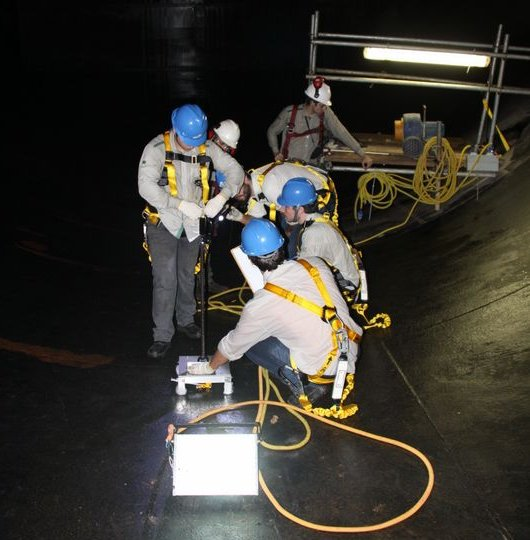
\includegraphics[width=0.6\columnwidth]{figs/base}
\caption{Teste de campo com a base  magnética}
\end{figure}

\noindent
\textbf{3500 Realização dos testes destrutivos – 1}
Realização dos testes para verificar se o revestimento mantém as 
características técnicas exigidas para a aplicação após mudanças de parâmetros. Nessa etapa foram realizados os testes de qualificação dos revestimentos antes e após mudanças de parâmetros e realização de ensaios destrutivos comparativos normatizados. 

\noindent
\textbf{3600 Aperfeiçoamento da solução:}
Aperfeiçoamento da solução baseado nos resultados dos testes de campo 

Tarefa atrasada em 1 mês com impacto de atraso de 1 mês no projeto. O cálculo da
posição relativa entre o robô e a pá, baseado em dados reais do sensor de
metrologia testado em campo, está com um erro de 0,1-0,2 graus o que resulta em
um erro de posição da extremidade do manipulador na ordem de centímetros. A
ordem de grandeza desejada para poder fazer reparo do perfil hidráulico é em
milímetros. Logo, as técnicas de alinhamento continuando sendo aprimoradas.

\begin{figure}\centering
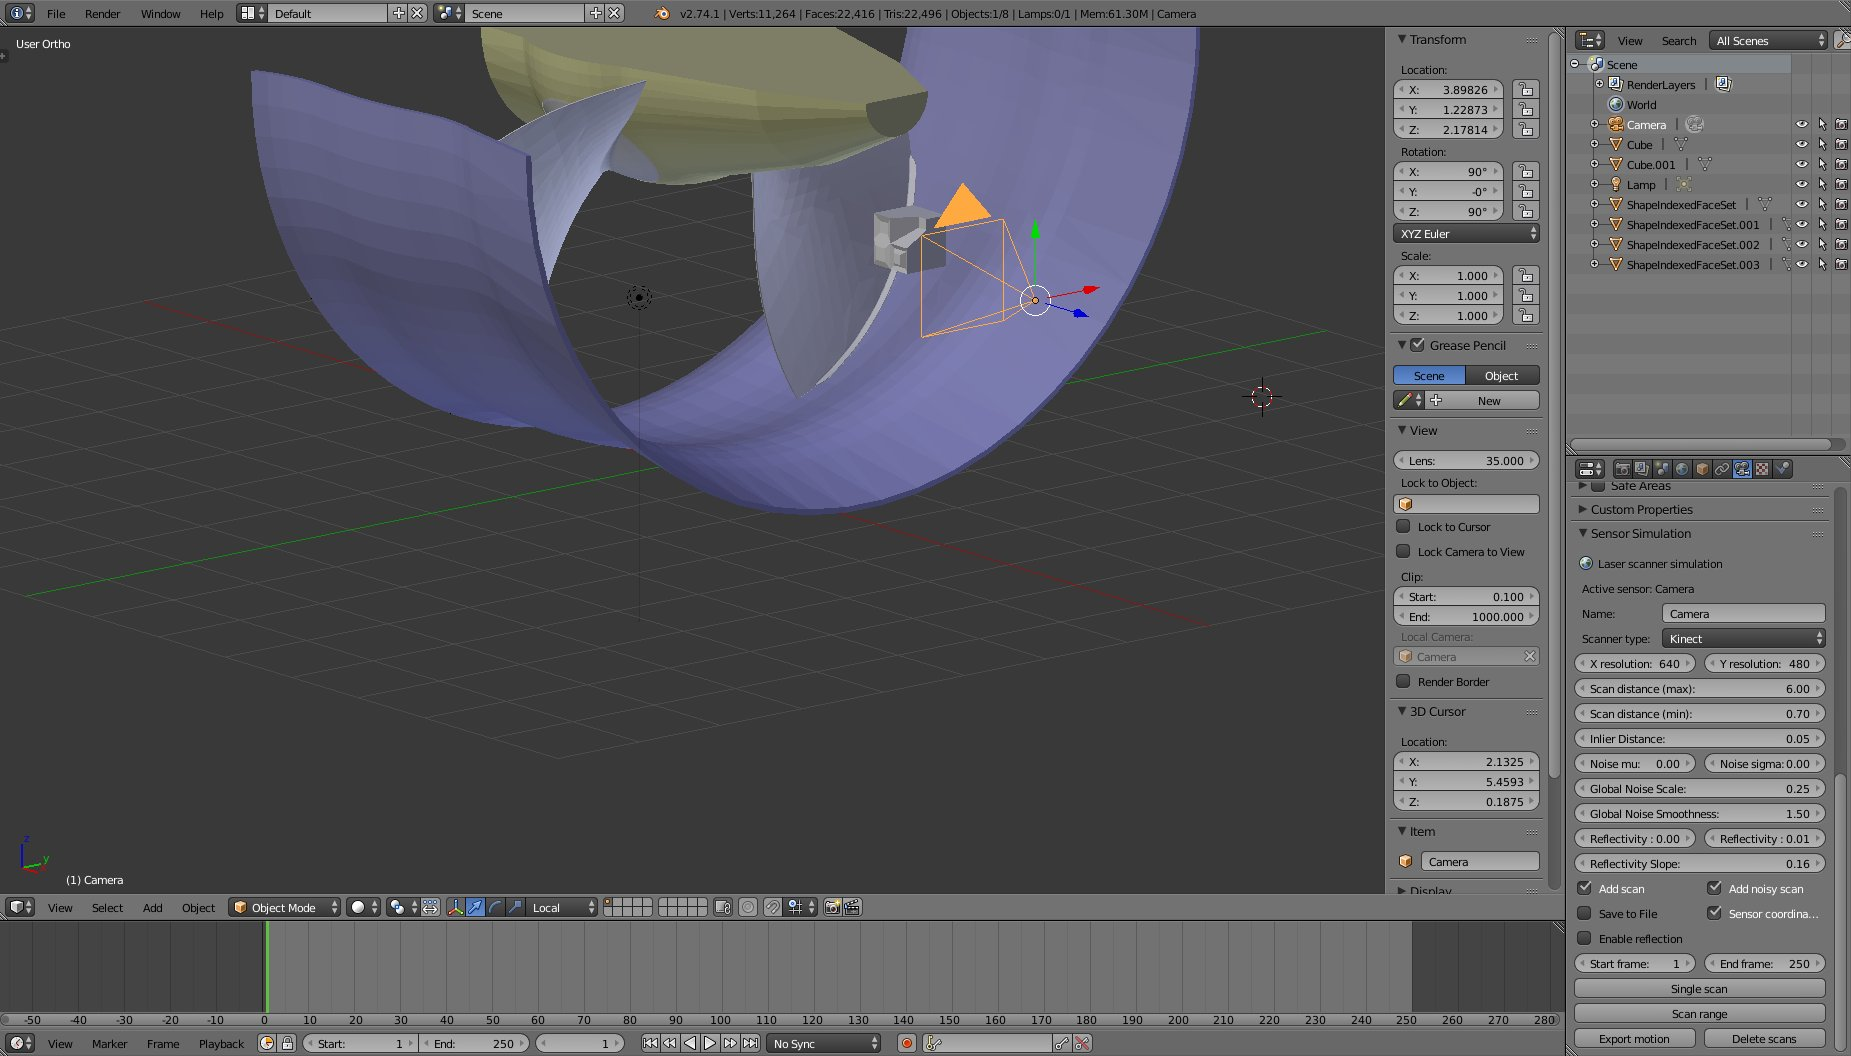
\includegraphics[width=0.6\columnwidth]{figs/blensor_screen}
\caption{Estimando posição relativa usando um simulador para análise dos
resultados.}
\end{figure} 


\noindent
\textbf{3700  Visita a campo para Inspeção 4:}
A inspeção nas pás é realizada com o fim de avaliar o progresso do desgate nas superfícies das pás e também determinar o tipo e a severidade em cada região da pá. 

\noindent
\textbf{3800 Realização dos testes destrutivos 2:}

Continuação da realização dos testes destrutivos após anális dos resultados prévio. As amostras que estvam em atraso na antrega dos resultados de cavitação foram realizadas nessa etapa. Também foram testes de aplicação de revestimento orgânico para melhoria das características do revestimento.


\noindent
\textbf{3900 Teste de Campo Jirau 02:} Teste da solução  em Jirau sobre
condições reais de operação.

Tarefa cancelada. As informações necessárias para esta fase do
projeto foram coletadas durante o teste de campo 01. 

\section{Etapa 04} 

\begin{figure}[H]
\centering
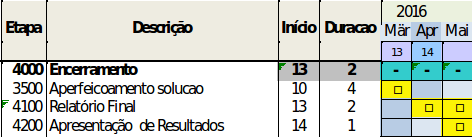
\includegraphics[width=0.7\columnwidth]{figs/etapa4}
\end{figure} 

\noindent
\textbf{4000 Encerramento:} A etapa 4000 do projeto foi executada existindo
variações entre previsto e executado. Inicialmente esta etapa era para ser
iniciada em março e encerrada em abril. Entretanto a mesma sofreu um atraso de 1
mês devido a necessidade de mais tempo para encerrar a etapa de aperfeiçoamento
da solução. O objetivo da etapa é preparar os relatórios finais e artigos acadêmicos do projeto.

\noindent
\textbf{4100 Relatório Final:} Relatório de encerramento do projeto no formato
P\&D Aneel e artigos acadêmicos.

Etapa executada como prevista. 

\noindent
\textbf{4200 Apresentação dos resultados:} Difusão dos conhecimentos.

Etapa executada como prevista. Foi realizado um evento na faculdade de Porto
Velho, onde os pesquisadores do projeto EMMA realizaram uma aula de pesquisa
aplicada explicando as pesquisas desenvolvidas, seus conceitos e resultados.
 

% ---------------------------------------------------------------------------
\chapter{Relatório Quadrimestral 1}
\includepdf[pages=1-,
addtotoc={1,section,1,Introdução,rq11[,1,section,1,Descrição do Problema,
rq1_2[,2,subsection,2,Descrição do
processo
HVOF,rq1_21[,3,subsection,2,Descrição dos
requisitos de operação de HVOF,rq1_22[,3,subsubsection,3,Jateamento da
superfície da pá,
rq1_221[,3,subsubsection,3,Reparo de danos
existentes,rq1_222[,3,paragraph,4,Reparo
com materiais não fundidos à
superfície,rq1_2221[,3,paragraph,4,Reparo
por solda,rq1_2222[,3,paragraph,4,Reparo por
solda e placa
sólida,rq1_2223[,4,subsection,2,Contextualização
do
ambiente,rq1_23[,4,subsubsection,3,Hélice
e pás,rq1_231[,4,subsubsection,3,Aro Câmara e regiões
adjacentes,rq1_232[,5,subsubsection,3,Escotilhas
de acesso,rq1_233[,5,subsubsection,3,Tubo de
sucção,rq1_234[,5,subsubsection,3,Infraestrutura
disponível,rq1_235[,6,subsection,2,Descrição das
tarefas do robô,rq1_24[,6,section,1,Estado da
arte,rq1_3[,6,subsection,2,Robôs sobre
trilhos,rq1_31[,7,subsection,2,Robôs
escaladores,rq1_32[,9,subsection,2,Robôs
cabeados,rq1_33[,10,subsection,2,Manipulador com
base esférica,rq1_34[,11,section,1,Projeto de
robô autônomo para
HVOF,rq1_4[,11,subsection,2,Acesso pela
escotilha
superior,rq1_41[,11,subsection,2,Acesso pela
escotilha
inferior,rq1_42[,12,subsubsection,3,Projeto
de robôs em trilhos,
rq1_421[,12,subsubsection,3,Projeto de
robôs
escaladores,rq1_422[,13,subsubsection,3,Projetos
com manipuladores industriais
fixos,rq1_423[,14,subsection,2,Solução
conceitual,rq1_43[,14,section,1,Estudo
de bases para manipuladores
industriais,rq1_5[,14,subsection,2,Modelagem
3D das soluções
conceituais,rq1_51[,15,subsubsection,3,Dimensionamento
da
base,rq1_511[,17,section,1,Conclusão
e trabalhos
futuros,rq1_6[,18,section,1,Referências,rq1_7]]]]]]]]]]]]]]]]]]]]]]]]]]]]]]]}]{pdfs/sota}
% ---------------------------------------------------------------------------

\chapter{Relatório Quadrimestral 2}
\includepdf[pages=1-,
addtotoc={1,section,1,Introdução,rq2_1[,1,section,1,Estudo de viabilidade
técnica detalhada,
rq2_2[,2,subsection,2,Pesquisa de
mercado,rq2_21[,2,subsection,2,Estudo
puramente geométrico,rq2_22[,2,subsubsection,3,KR 10 R1100 sixx WP (Kuka),
rq2_221[,3,subsubsection,3,MH12
(Motoman),rq2_222[,3,subsection,2,Espaço de
trabalho e cinemática do
manipulador,rq2_23[,5,subsubsection,3,KR 10 R1100 sixx WP
(Kuka),rq2_231[,5,subsubsection,3,MH12
(Motoman),rq2_232[,5,subsubsection,3,LBR iiwa 14 R820
(Kuka),rq2_233[,6,subsubsection,3,SIA20D,rq2_234[,7,subsubsection,3,Tolerância
no ângulo de
revestimento,rq2_235[,8,subsection,2,Dinâmica do
manipulador,rq2_24[,9,subsection,2,Detalhamento
da base
mecânica,rq2_25[,10,subsubsection,3,Conceitos
de base mecânica,rq2_251[,11,subsubsection,3,Sistemas
de elevação fixação e
ancoragem,rq2_252[,12,subsection,2,Shutter,rq2_26[,12,section,1,Calibração,rq2_3[,12,subsection,2,Estudo
de sensores,rq2_31[,13,subsubsection,3,3D
scanners,rq2_311[,13,paragraph,4,Estações de
medição,rq2_3111[,13,paragraph,4,Velodyne,rq2_3112[,13,paragraph,4,Forecast
3D Laser system,rq2_3113[,13,subsubsection,3,ToF
Cameras,rq2_312[,14,paragraph,4,Mesa imaging swissranger sr400,
rq2_3121[,14,paragraph,4,Sentis M100 Argos
3D - P100,rq2_3122[,14,subsubsection,3,Câmeras
de luz
estruturado,rq2_313[,14,subsection,2,Conclusão,rq2_32[,14,subsubsection,3,Medidor
de distância a
laser,rq2_321[,15,paragraph,4,Temperatura,rq2_3211[,15,paragraph,4,Distância
de
operação,rq2_3212[,15,paragraph,4,Poeira
e
umidade,rq2_3213[,15,paragraph,4,Precisão,rq2_3214[,15,paragraph,4,Peso,rq2_3215[,16,subsection,2,Estudo
de técnicas de
reconhecimento,rq2_33[,16,subsubsection,3,Reconhecimento
do
robô,rq2_331[,16,paragraph,4,RANSAC,rq2_3311[,16,paragraph,4,Transformada
de Hough
3D,rq2_3212[,17,subsubsection,3,Reconhecimento
da
pá,rq2_332[,19,section,1,Interfaces
de
usuários,rq2_4[,19,subsection,2,Pesquisa
de
usuário,rq2_41[,19,subsection,2,Análise
de
tarefas,rq2_42[,19,subsubsection,3,Calibração,rq2_421[,19,subsubsection,3,Planejamento
de
trajetória,rq2_422[,19,subsubsection,3,Metalização,rq2_423[,19,subsection,2,Casos
de uso,rq2_43[,19,subsection,2,Design conceitual,rq2_44[,19,subsection,2,Estrutura
de testes de
usabilidade,rq2_45[,19,section,1,Conclusão
e trabalhos
futuros,rq2_5]]]]]]]]]]]]]]]]]]]]]]]]]]]]]]]]]]]]]]]]]]]}]{pdfs/detail}
% ---------------------------------------------------------------------------

\chapter{Relatório Quadrimestral 3}
\includepdf[pages=1-,
addtotoc={1,section,1,Introdução,rq3_1[,1,section,1,Metodologia do sistema de
controle, rq3_2[,2,subsection,2,Construção do
ambiente de
simulação,rq3_21[,2,subsection,2,Análises
cinemática dinâmica e controle do
manipulador,rq3_22[,2,subsubsection,3,Avaliação dos extremos da pá,
rq3_221[,2,paragraph,4,Extremidade inferior
esquerda,rq3_2211[,3,paragraph,4,Extremidade
inferior
direita,rq3_2212[,3,paragraph,4,Extremidade
superior
esquerda,rq3_2213[,3,paragraph,4,Extremidade
superior
direita,rq3_2214[,4,paragraph,4,Conclusão
da
simulação
de
extremidades,rq3_2215[,4,subsubsection,3,Teste
de revestimento completo e novas soluções
de base,rq3_222[,4,paragraph,4,Extremidade
superior
esquerda,rq3_2221[,5,paragraph,4,Lateral
direita,rq3_2222[,5,paragraph,4,Extremidade
superior
direita,rq3_2223[,6,paragraph,4,Conclusão
da simulação
completa,rq3_2224[,6,subsection,2,Planejamento
de
trajetória,rq3_23[,6,subsubsection,3,Modelagem
da
superfície,rq3_231[,6,subsubsection,3,Cálculo dos
paralelos,rq3_232[,8,subsubsection,3,Cálculo dos
meridianos,rq3_233[,9,subsection,2,Conclusão,rq3_24[,9,section,1,Solução
mecânica,rq3_3[,9,subsection,2,Conceito,rq3_31[,10,subsection,2,Construção,rq3_32[,10,subsubsection,3,Trilho
e carrinho,rq3_321[,10,subsubsection,3,Perfil de alumínio,
rq3_322[,11,subsubsection,3,Pés de
apoio,rq3_323[,11,subsubsection,3,Ancoragem,rq3_324[,11,subsubsection,3,Bases
magnéticas,rq3_325[,12,subsubsection,3,Junta
de
rotação,rq3_326[,12,subsubsection,3,Junta de
elevação,rq3_327[,12,subsection,2,Dimensionamento,rq3_33[,13,subsubsection,3,Trilho,rq3_331[,13,subsubsection,3,Estrutura,rq3_332[,15,subsubsection,3,Base
magnética,rq3_333[,15,subsection,2,Conclusão,rq3_34[,15,section,1,Solução
da
calibração,rq3_4[,15,subsection,2,Reconhecimento
do
robô,rq3_41[,16,subsubsection,3,RANSAC,rq3_411[,16,subsubsection,3,Transformada
de hough 3D,rq3_412[,17,subsection,2,Calibração
da pá,rq3_42[,18,subsubsection,3,Correspondence
Grouping,rq3_421[,18,subsection,2,Simulação
de
nuvem
de
pontos,rq3_43[,18,subsubsection,3,Dados
genéricos,rq3_431[,18,subsubsection,3,Blensor,rq3_432[,20,subsection,2,Análise
de
resultados,rq3_44[,20,subsection,2,Conclusão,rq3_45[,21,section,1,Referências,rq3_5[,21,section,1,Apêndice,rq3_6]]]]]]]]]]]]]]]]]]]]]]]]]]]]]]]]]]]]]]]]]]}]{pdfs/method}
% ---------------------------------------------------------------------------

\chapter{Viagem Inaugural}

\includepdf[pages=1-]{pdfs/Viagem01_EMMA}
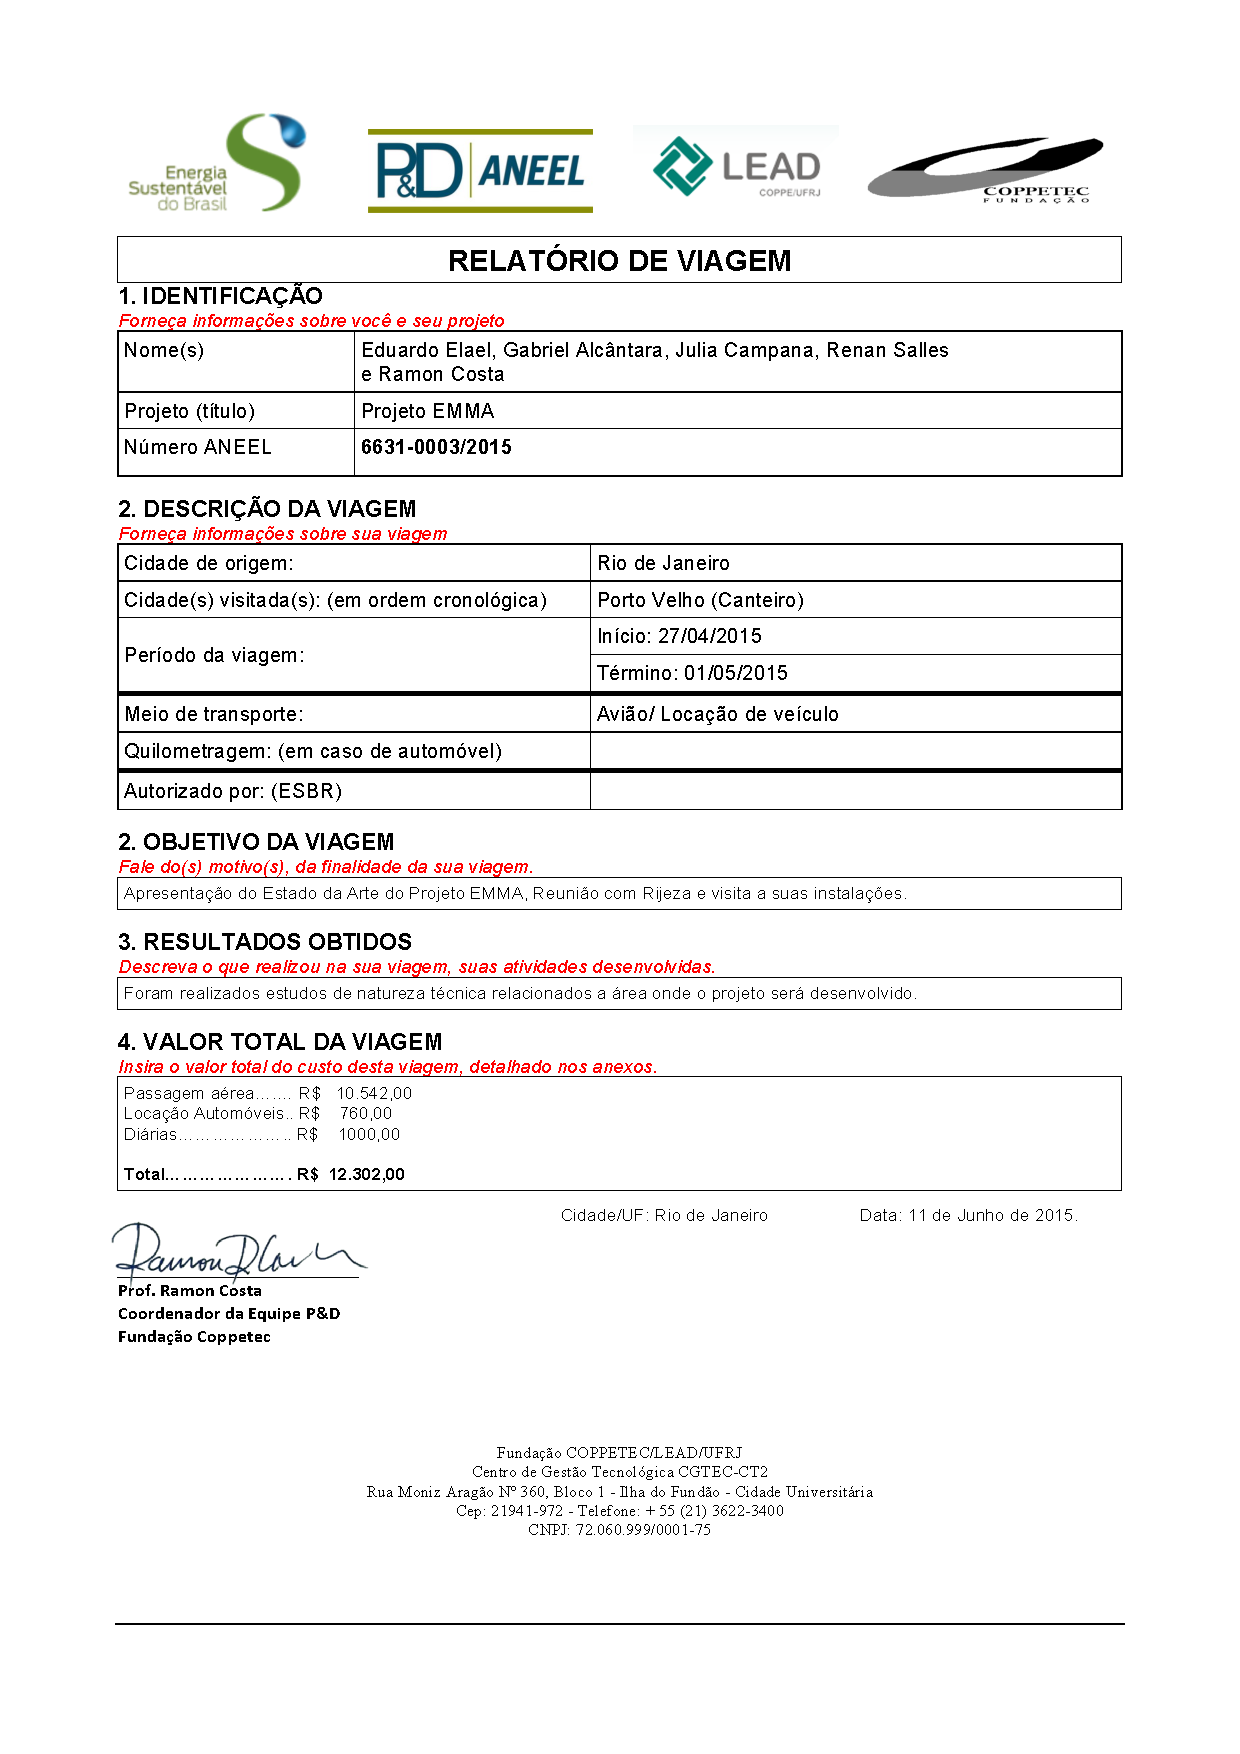
\includepdf[pages=1-]{pdfs/Viagem01_EMMA_ESBR}

\chapter{Viagem de reconhecimento Rijeza}
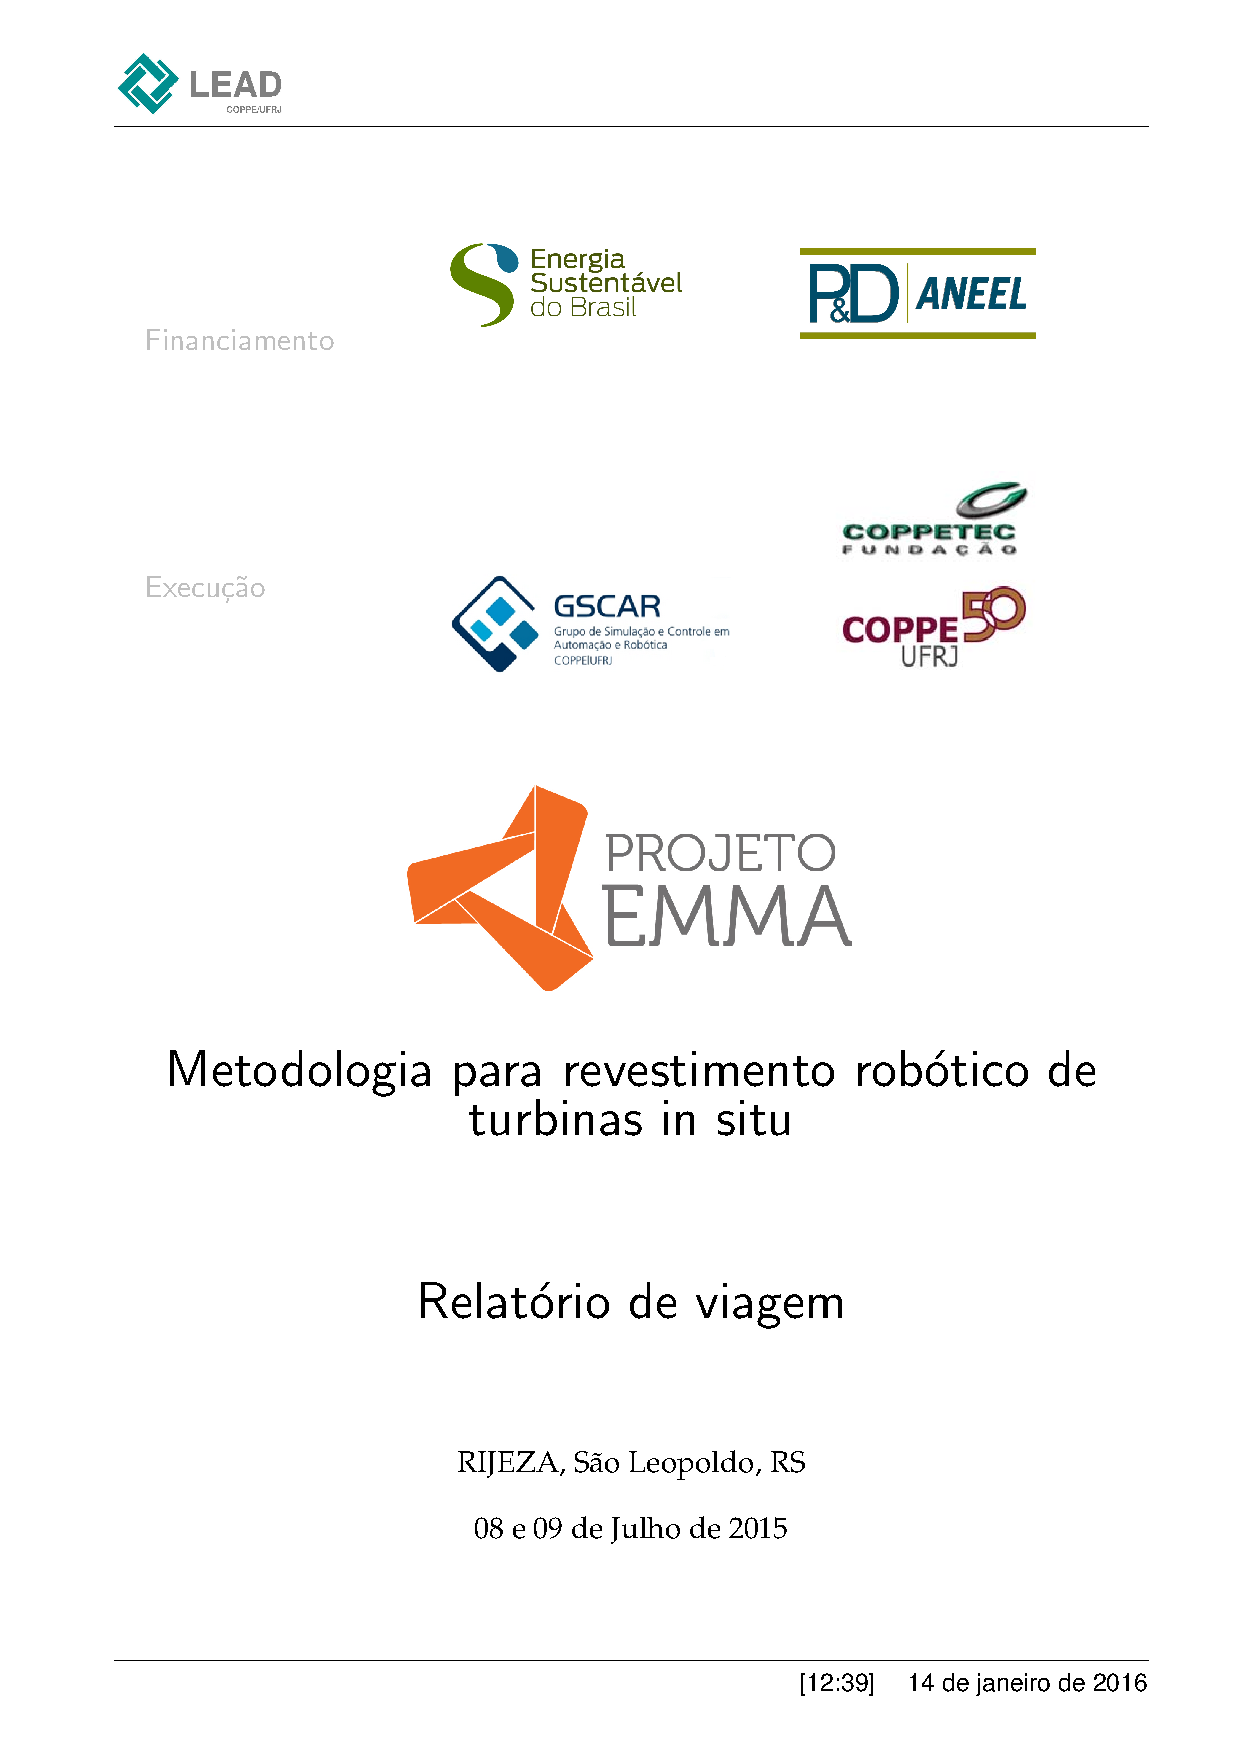
\includepdf[pages=1-]{pdfs/Viagem02_EMMA}
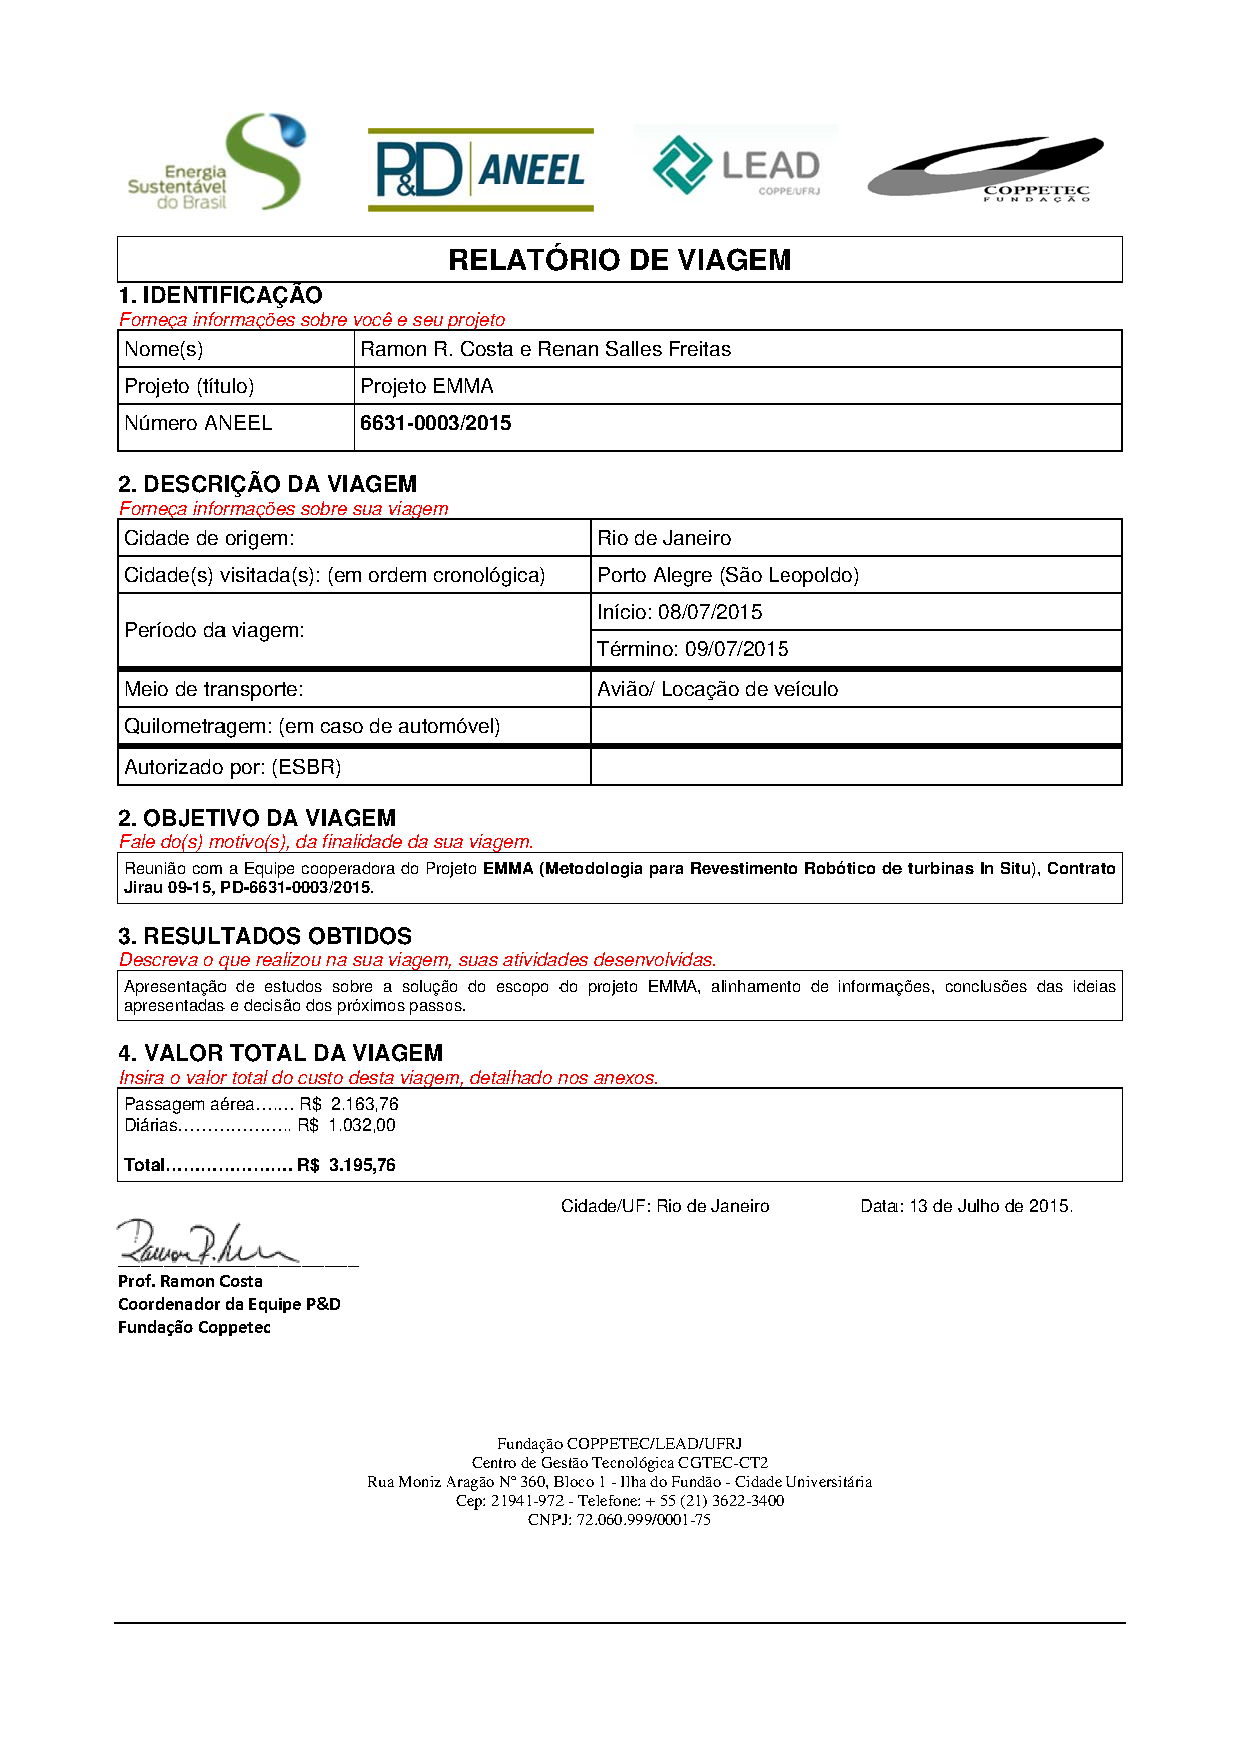
\includepdf[pages=1-]{pdfs/Viagem02_EMMA_ESBR}

\chapter{Viagem de testes de campo}
\includepdf[pages=1-]{pdfs/Viagem04_EMMA}
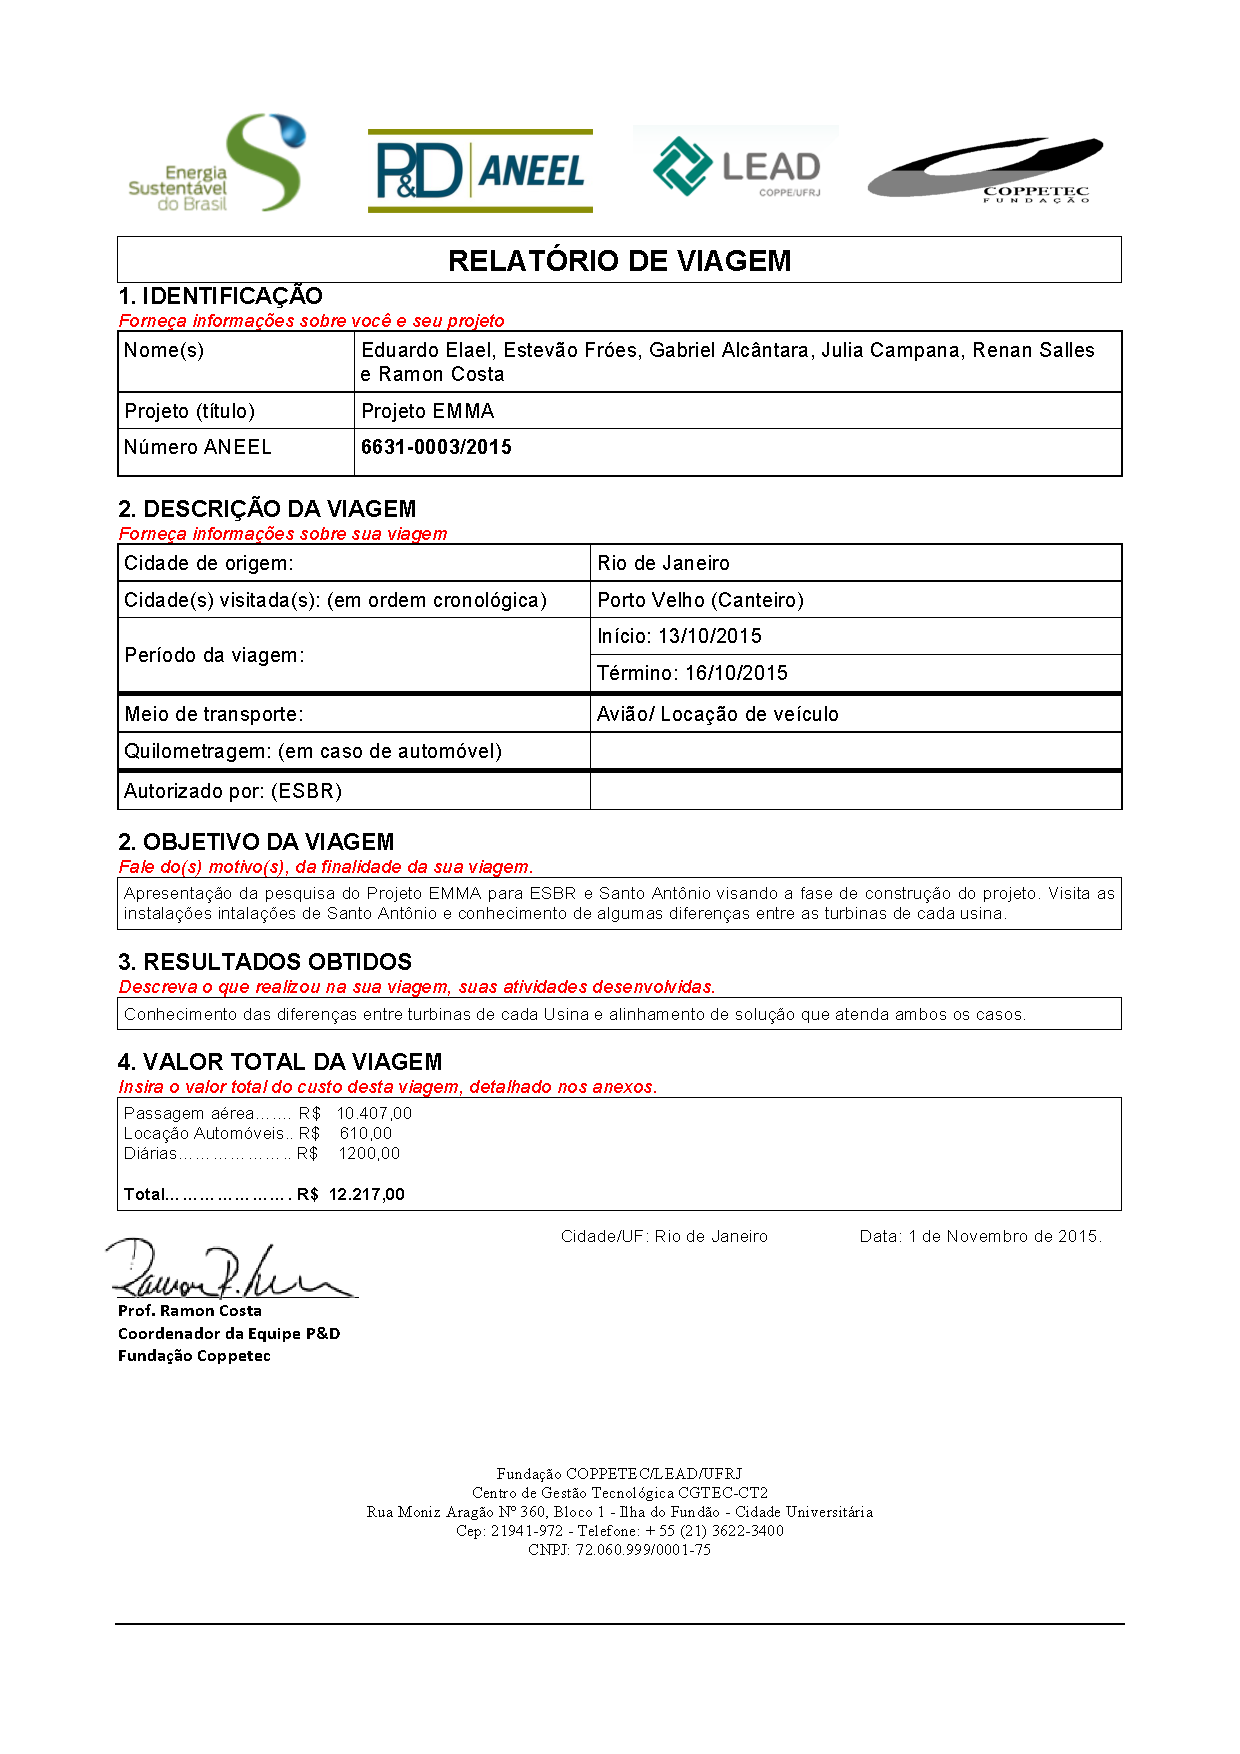
\includepdf[pages=1-]{pdfs/Viagem04_EMMA_ESBR}
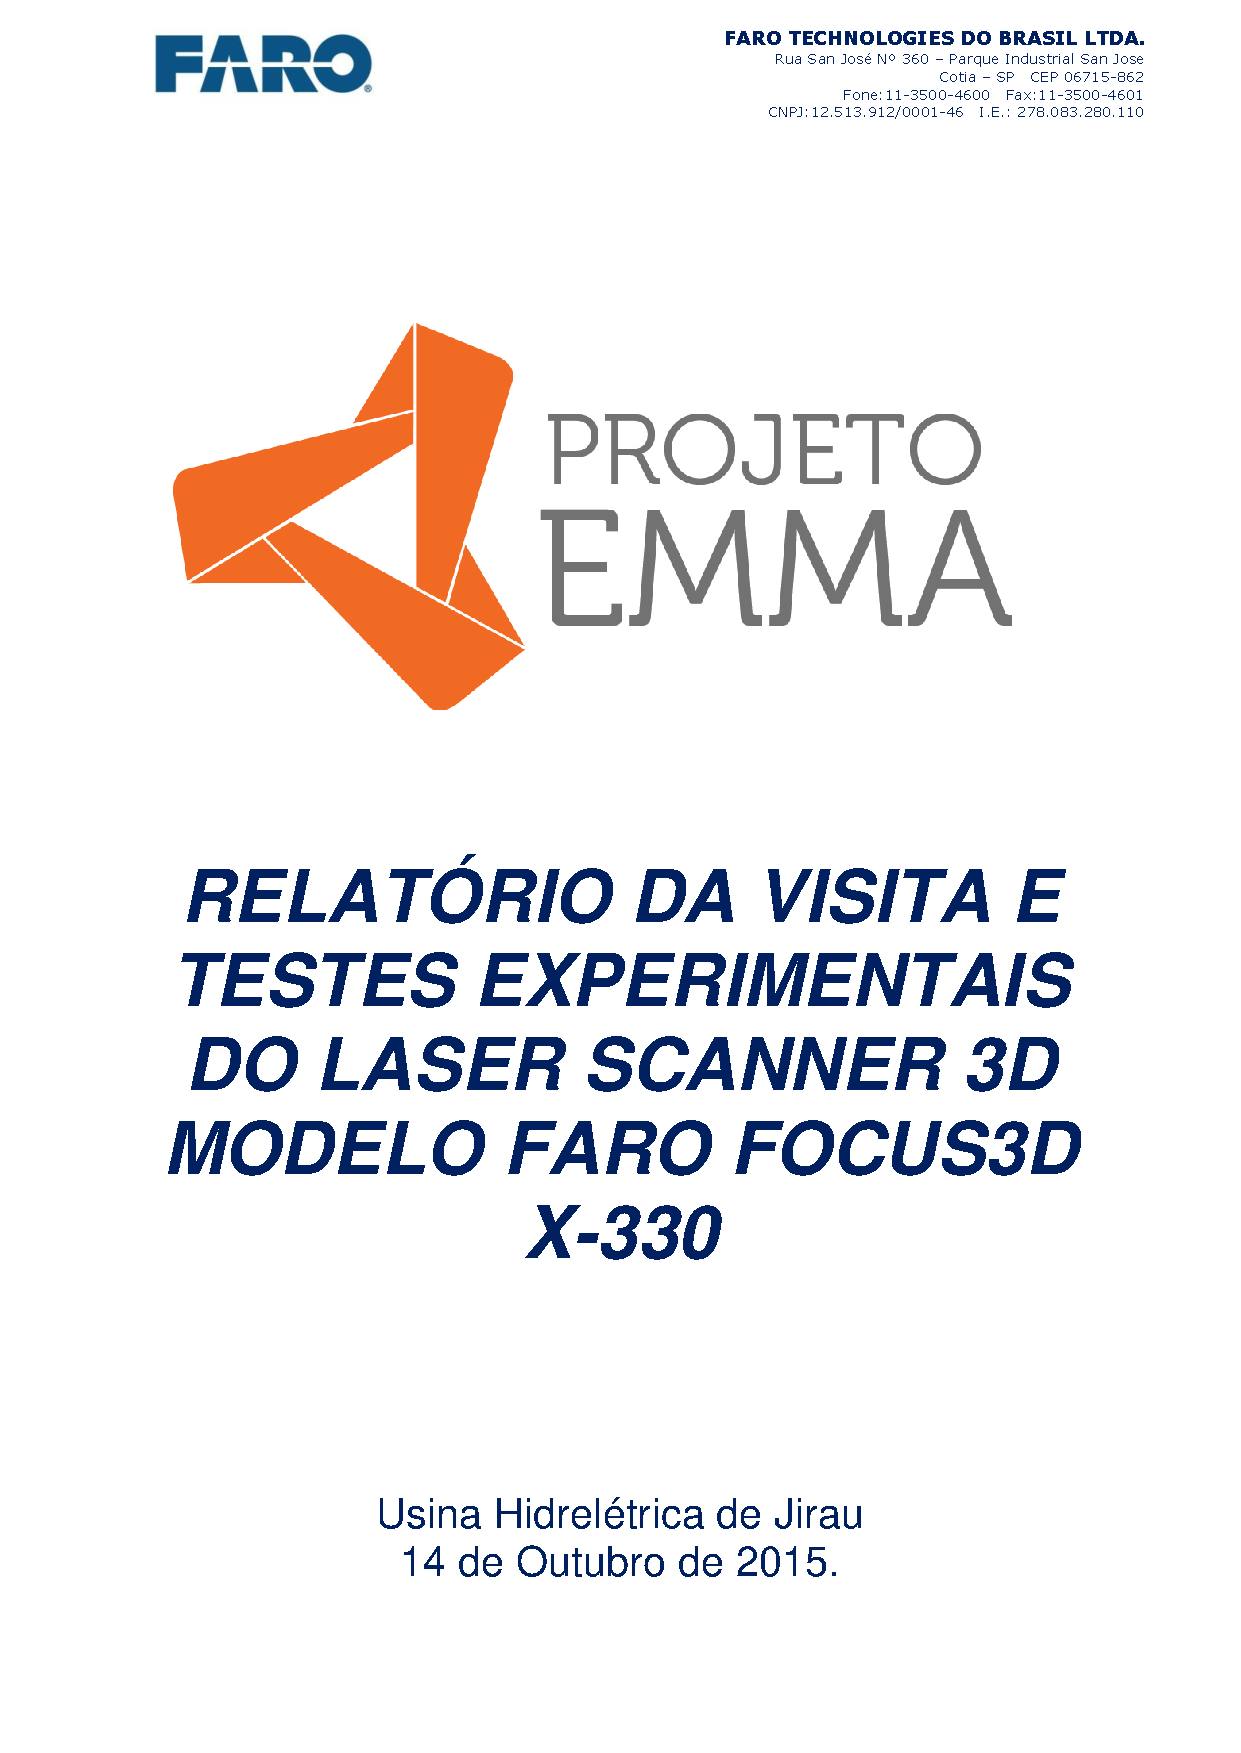
\includepdf[pages=1-]{pdfs/RelatorioFARO}

\chapter{Capacitação}
A pesquisa e o desenvolvimento (P\&D) tem como propósito fomentar o avanço
tecnológico e novas maneiras de desenvolver tipos específicos de conhecimento
no país. O desenvolvimento do robô EMMA, no âmbito P\&D é um exemplo de como a
parceria entre agências do governo e uni- versidades federais podem colaborar
para a capacitação tecnológica e o desenvolvimento de novas tecnologias.
Especificamente na área de robótica, o projeto EMMA mostra como a otimização e
automação de diversos processos de trabalho pode contribuir na indústria
energética. Em termos acadêmicos, esta linha de projetos possibilitou a
realização de duas
dissertações de mestrado, uma no Programa de Engenharia Elétrica (PEE),
Universidade Federal do Rio de Janeiro (UFRJ), e outra no Departamento
de Artes e Design (PPGDesign):%, abordando os seguintes tópicos:

%TODO Julia e Estevao - Propostas

%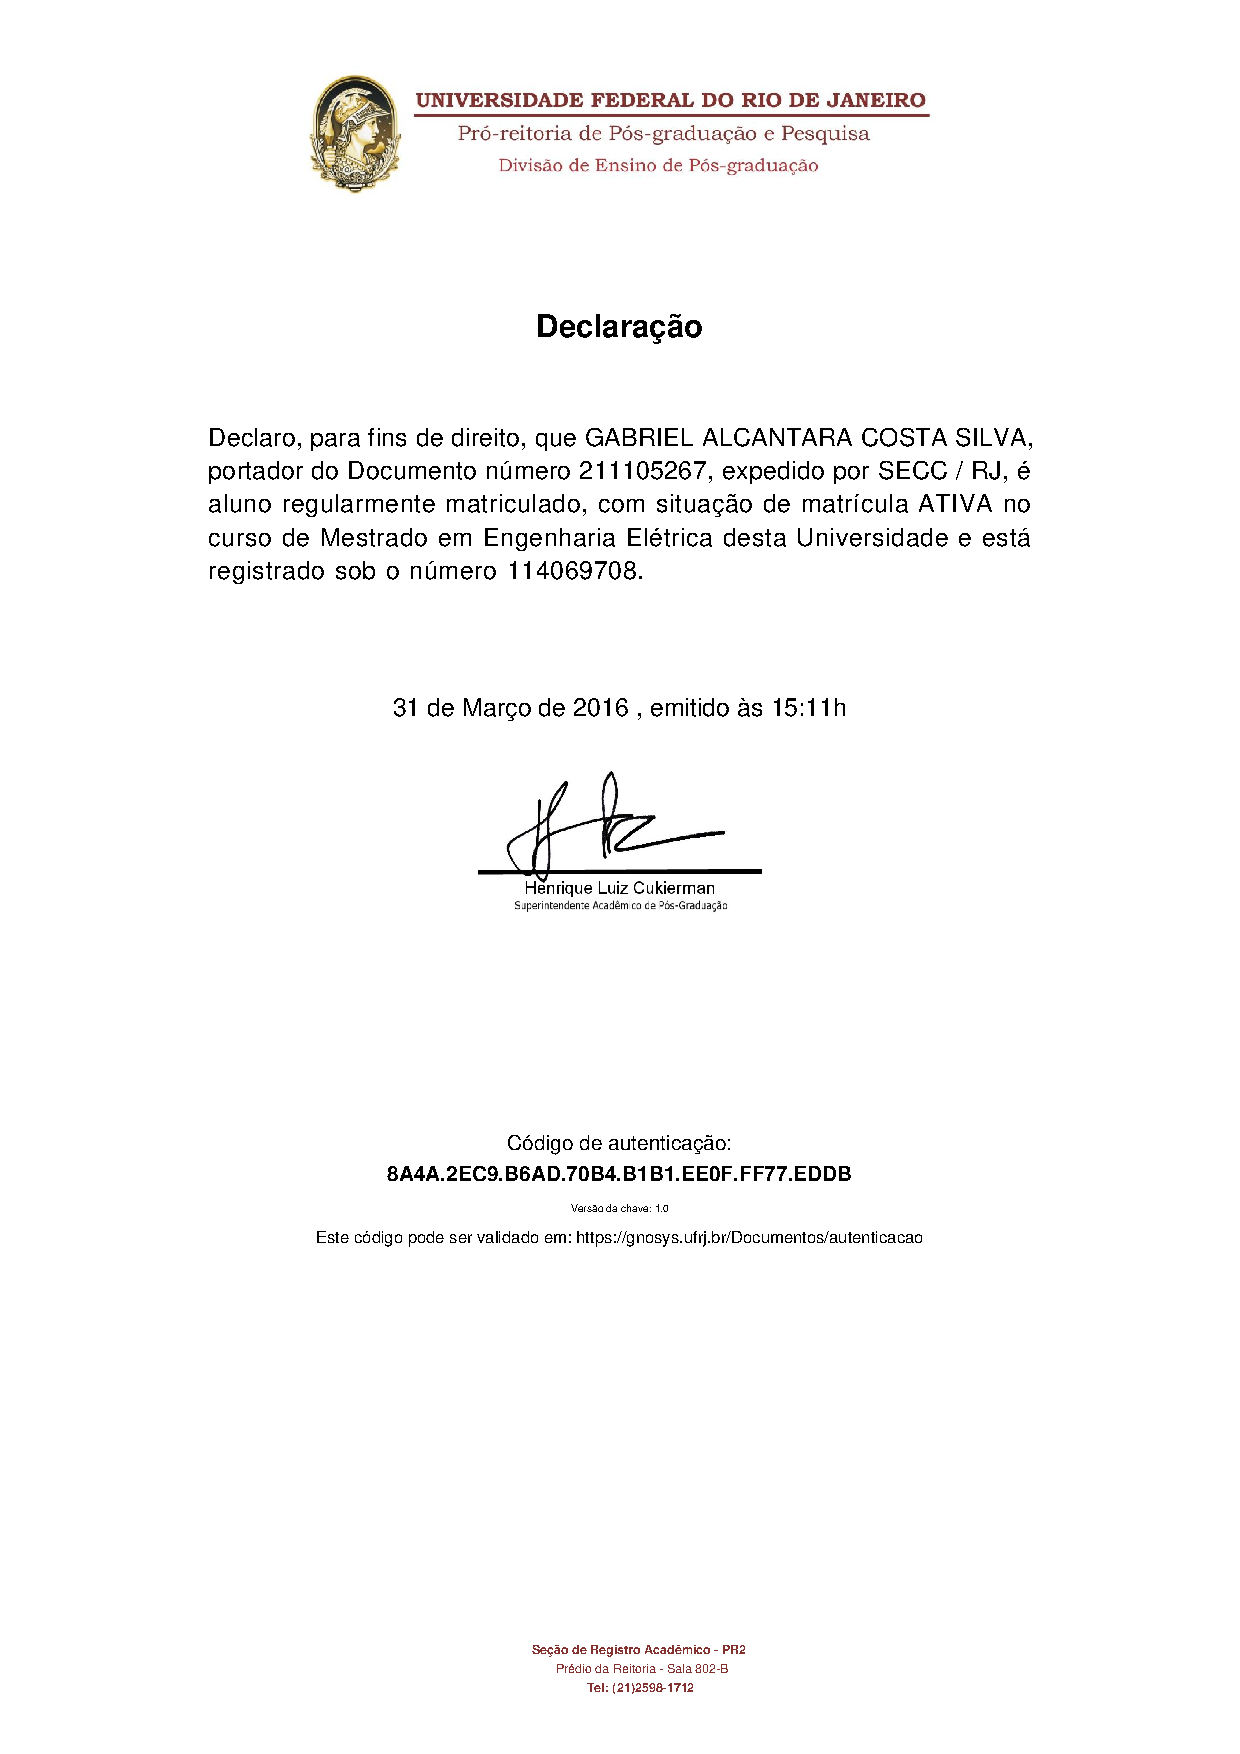
\includepdf{pdfs/mestrado_gabriel}
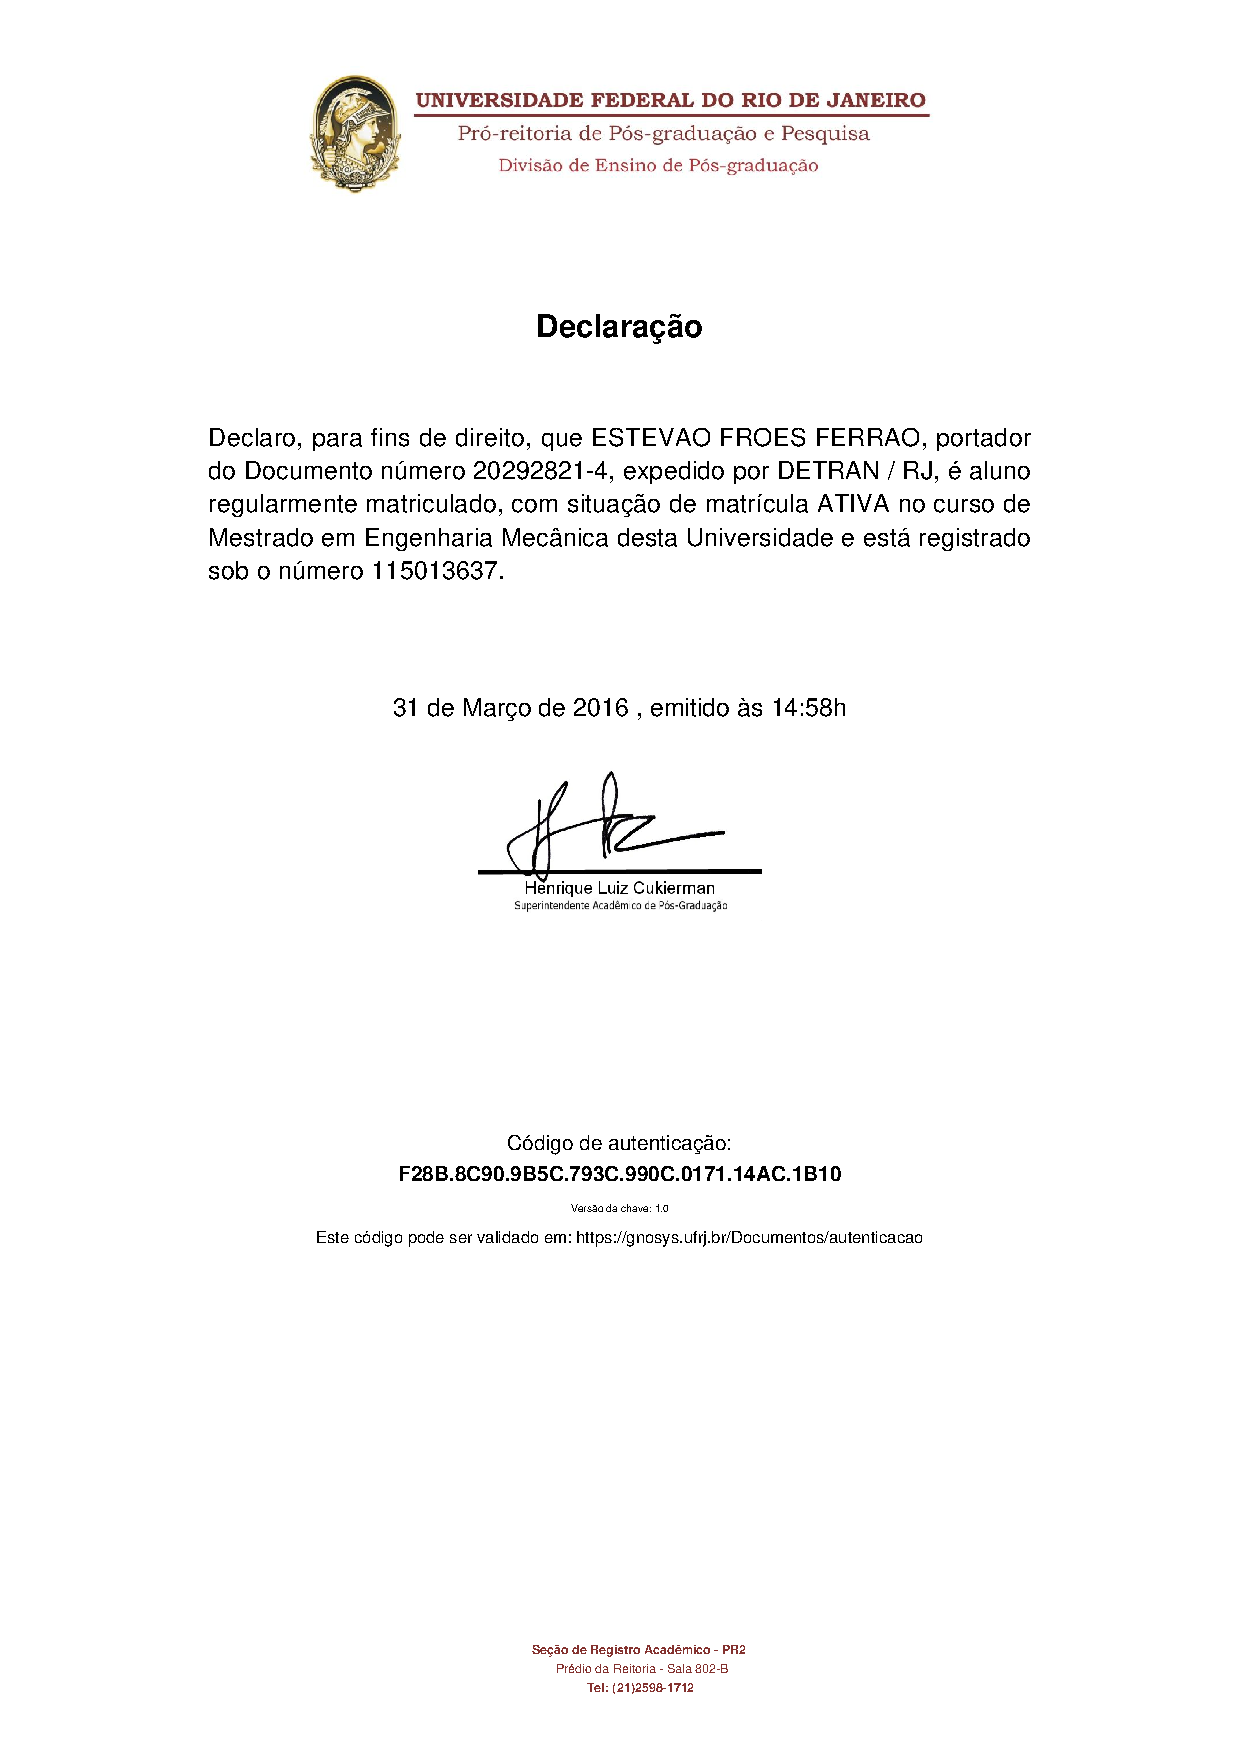
\includepdf{pdfs/mestrado_estevao}
%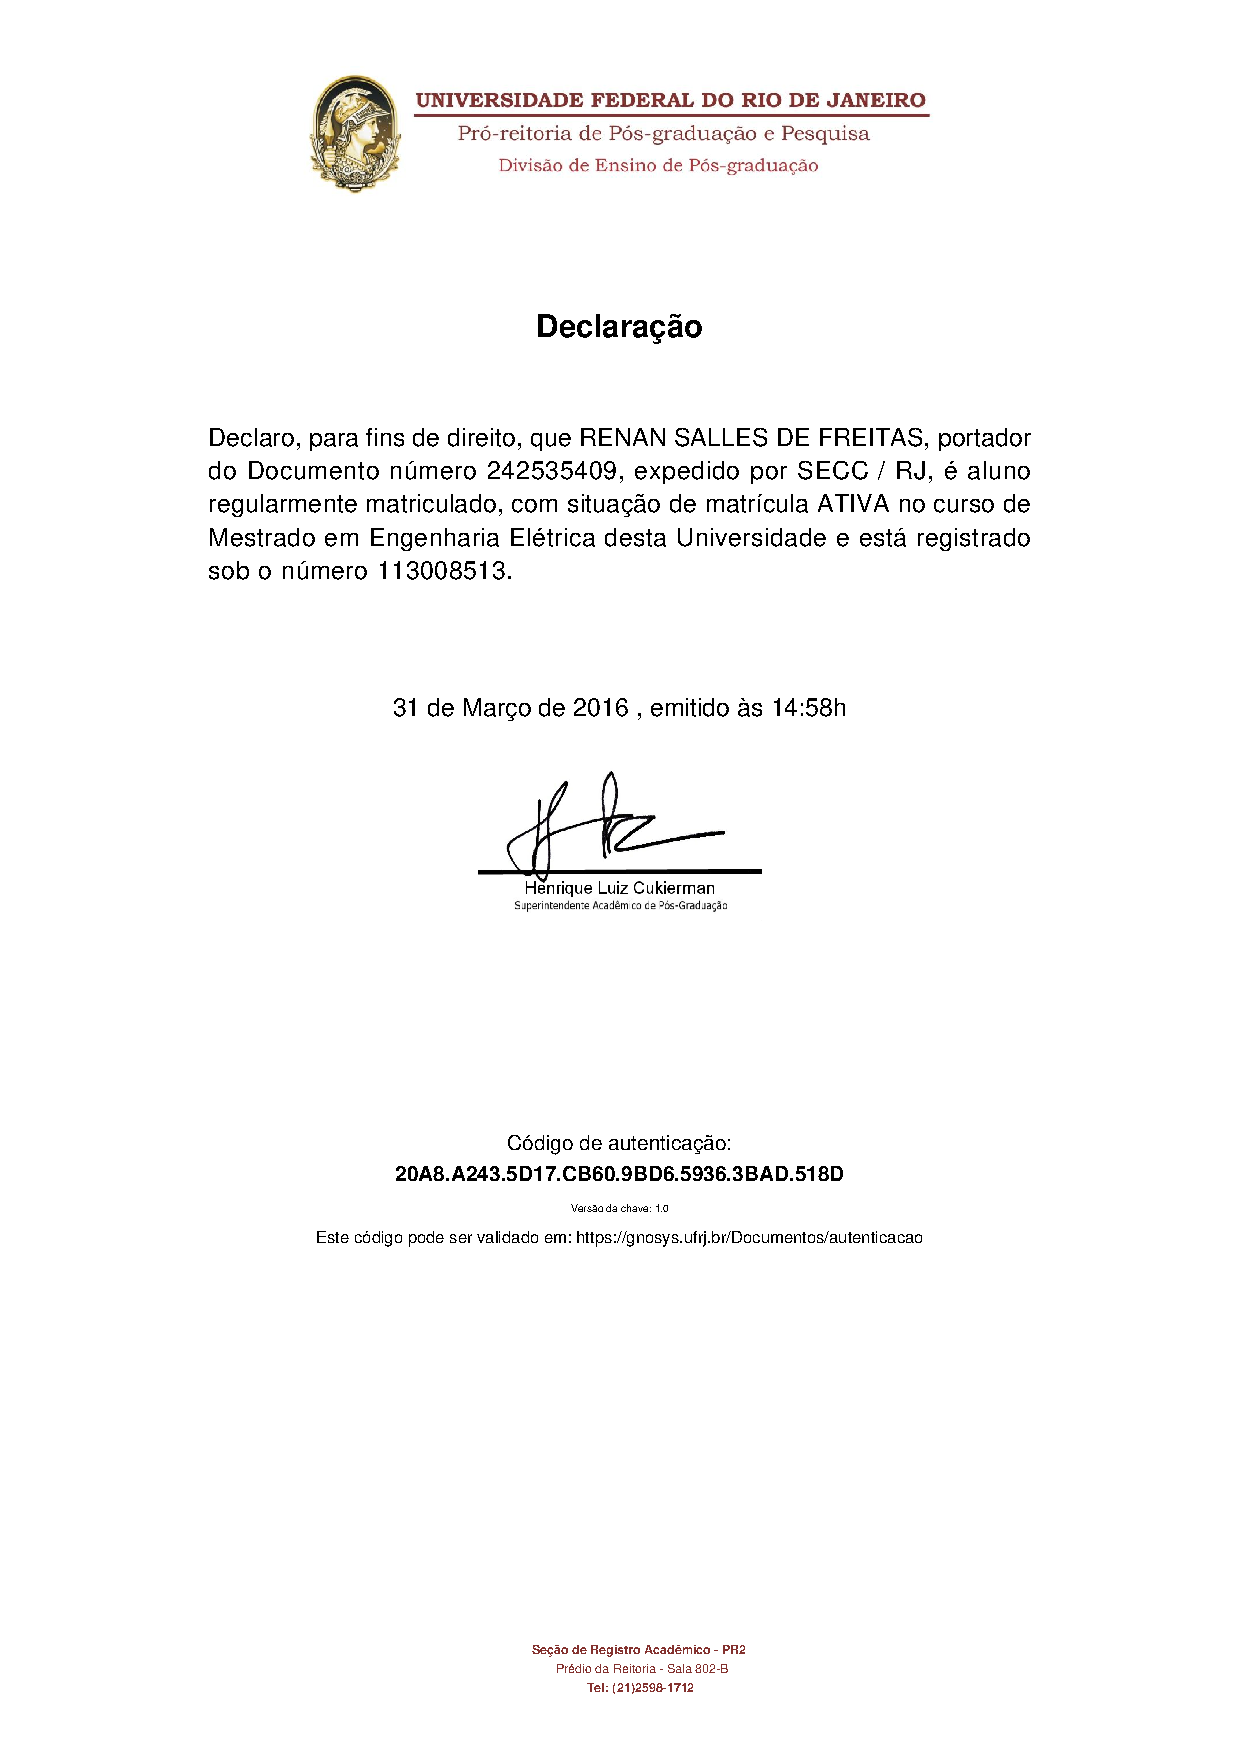
\includepdf{pdfs/mestrado_renan}
%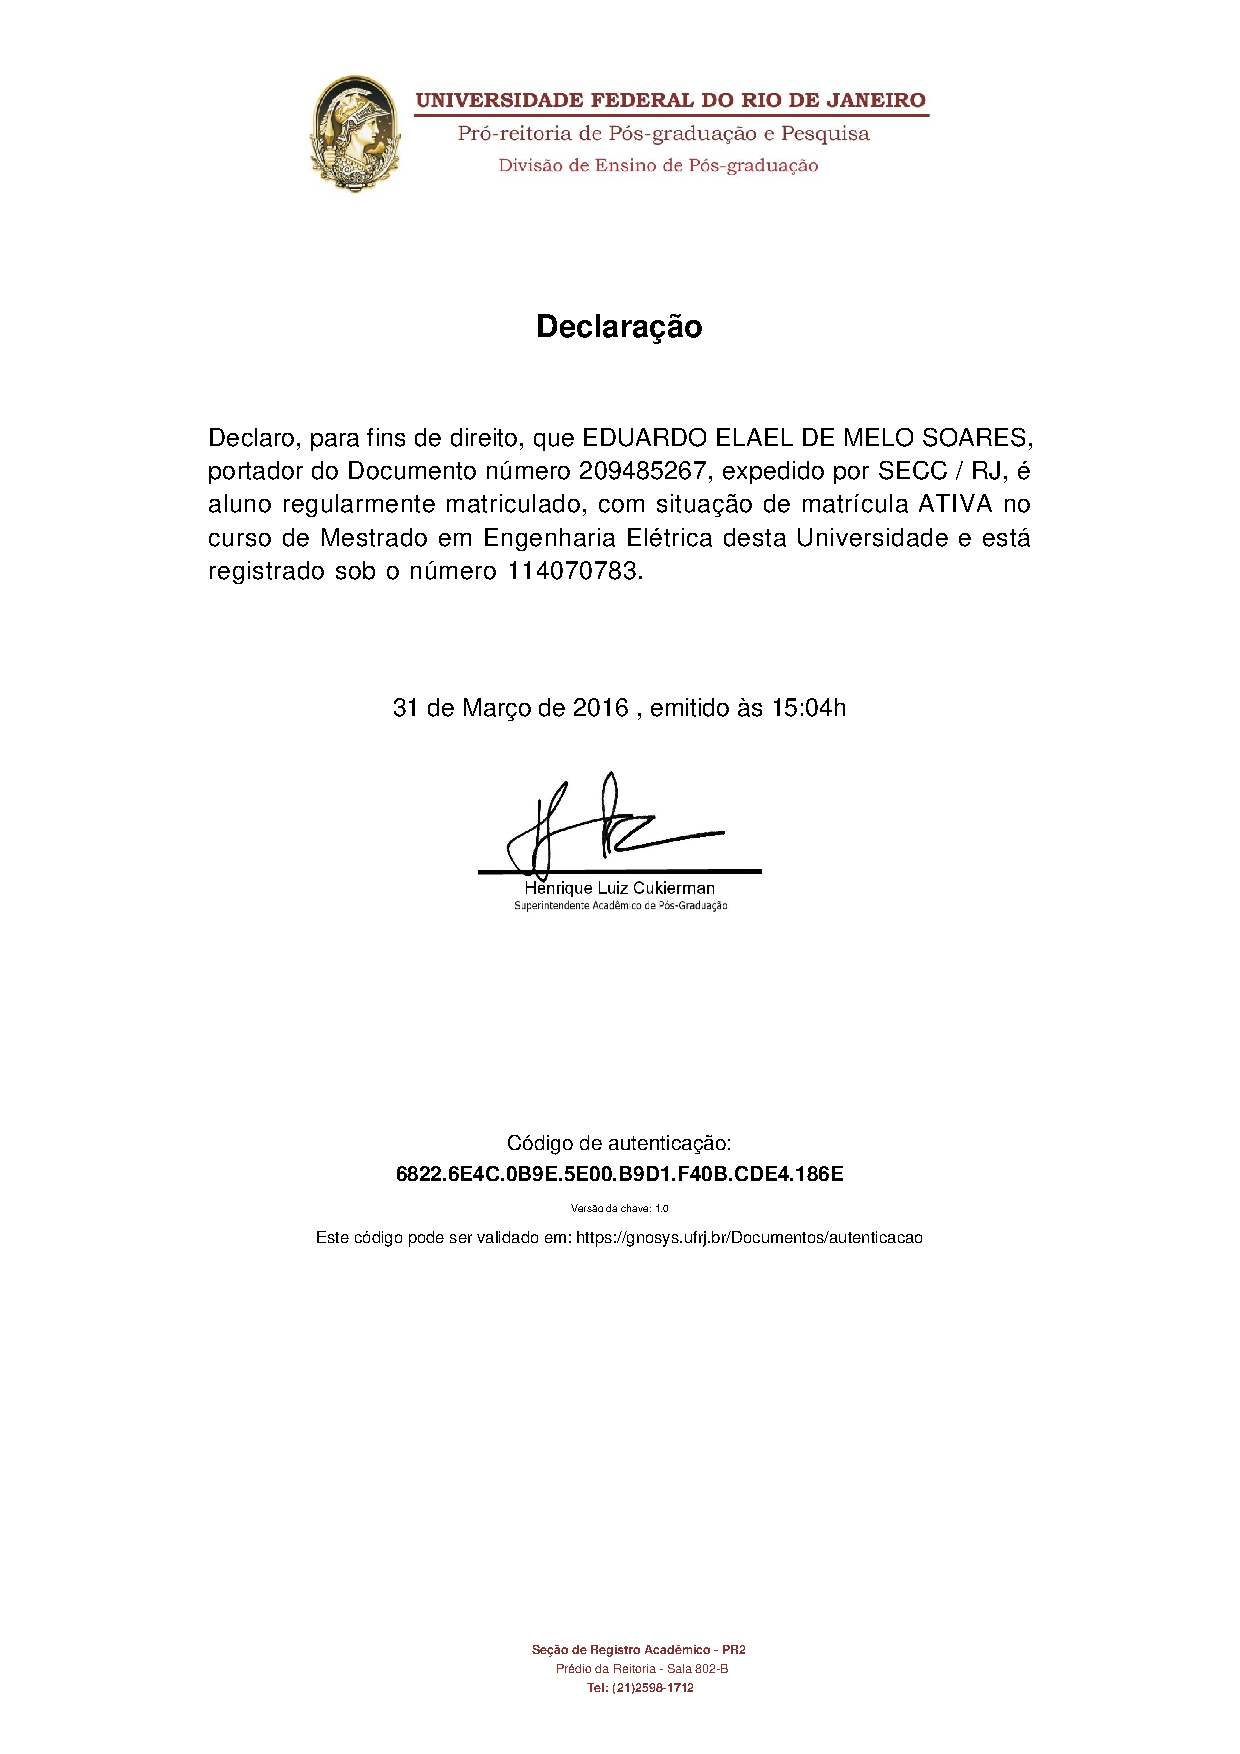
\includepdf{pdfs/mestrado_elael}
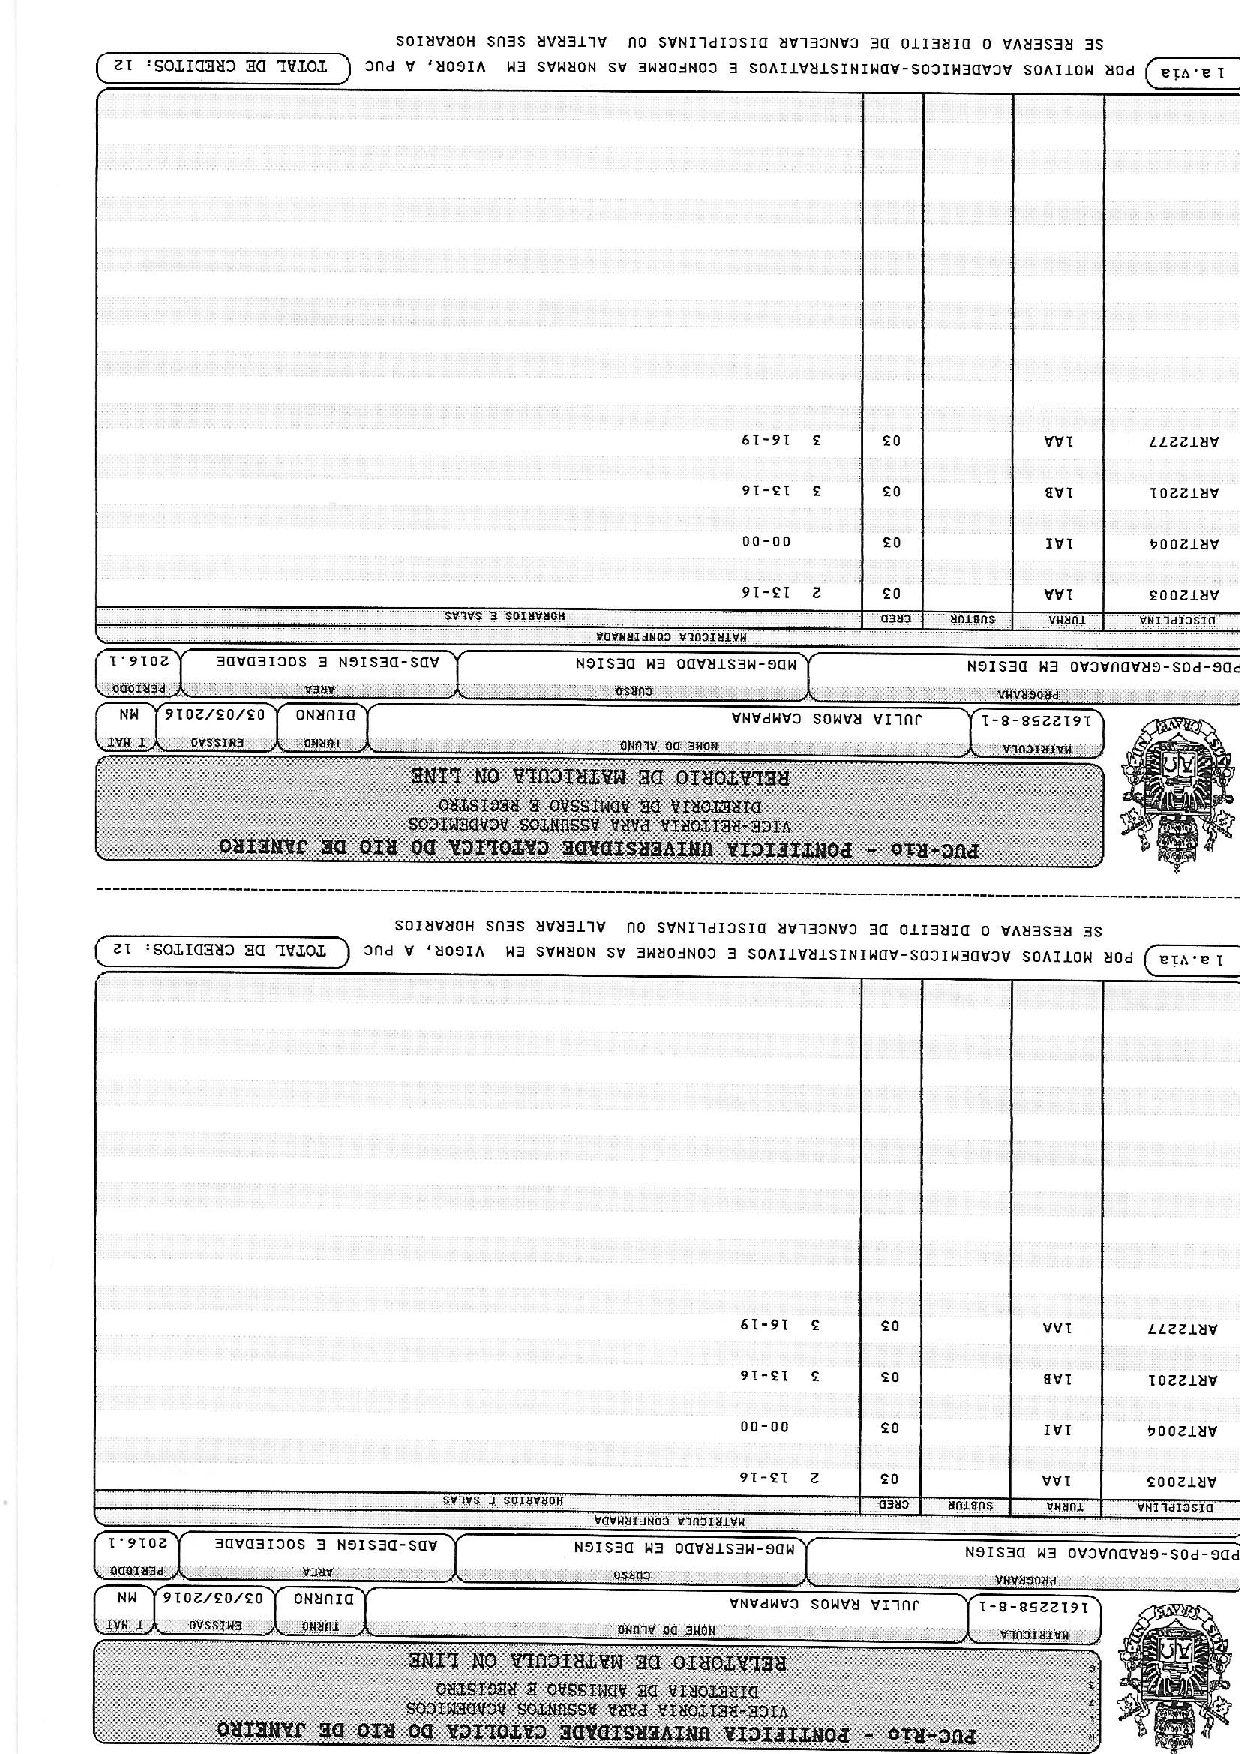
\includepdf[angle=180]{pdfs/mestrado_julia}

\chapter{Certificação}

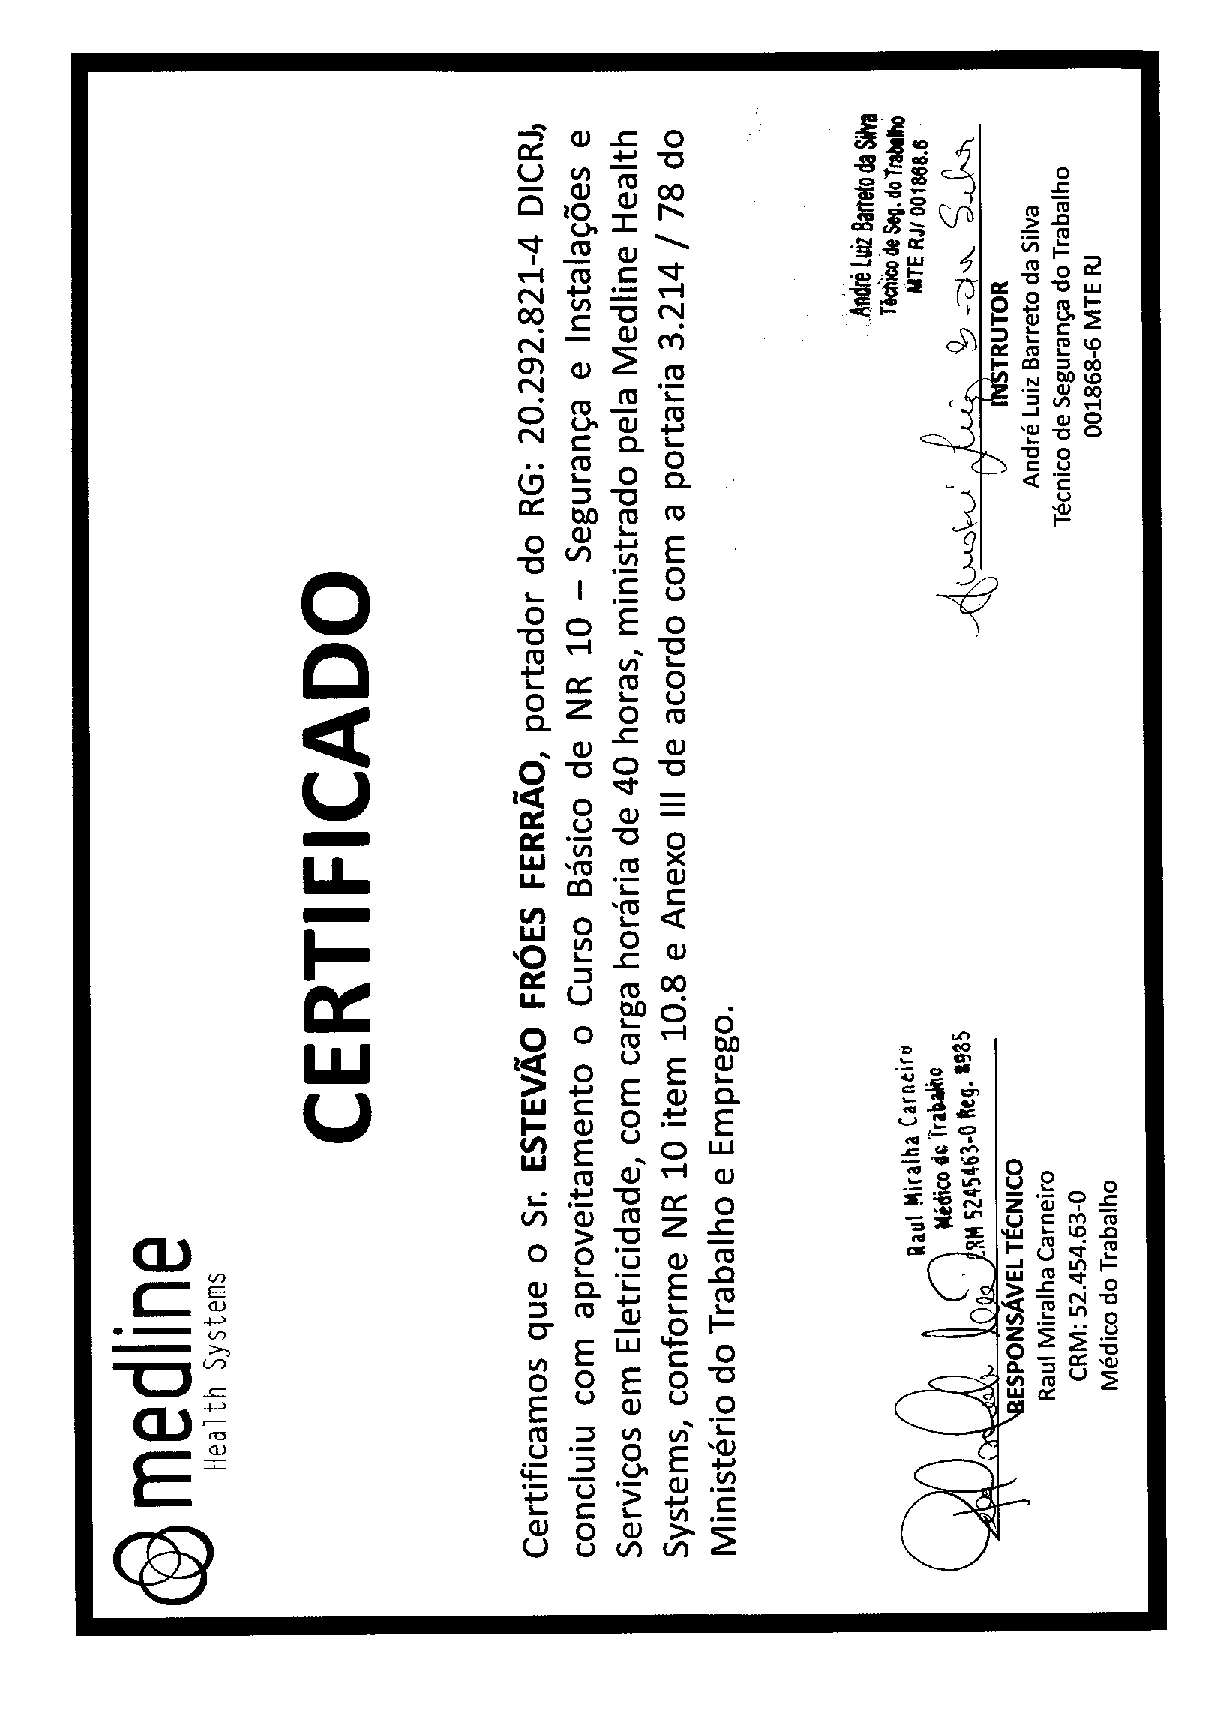
\includepdf[pages=1-]{pdfs/NR10}
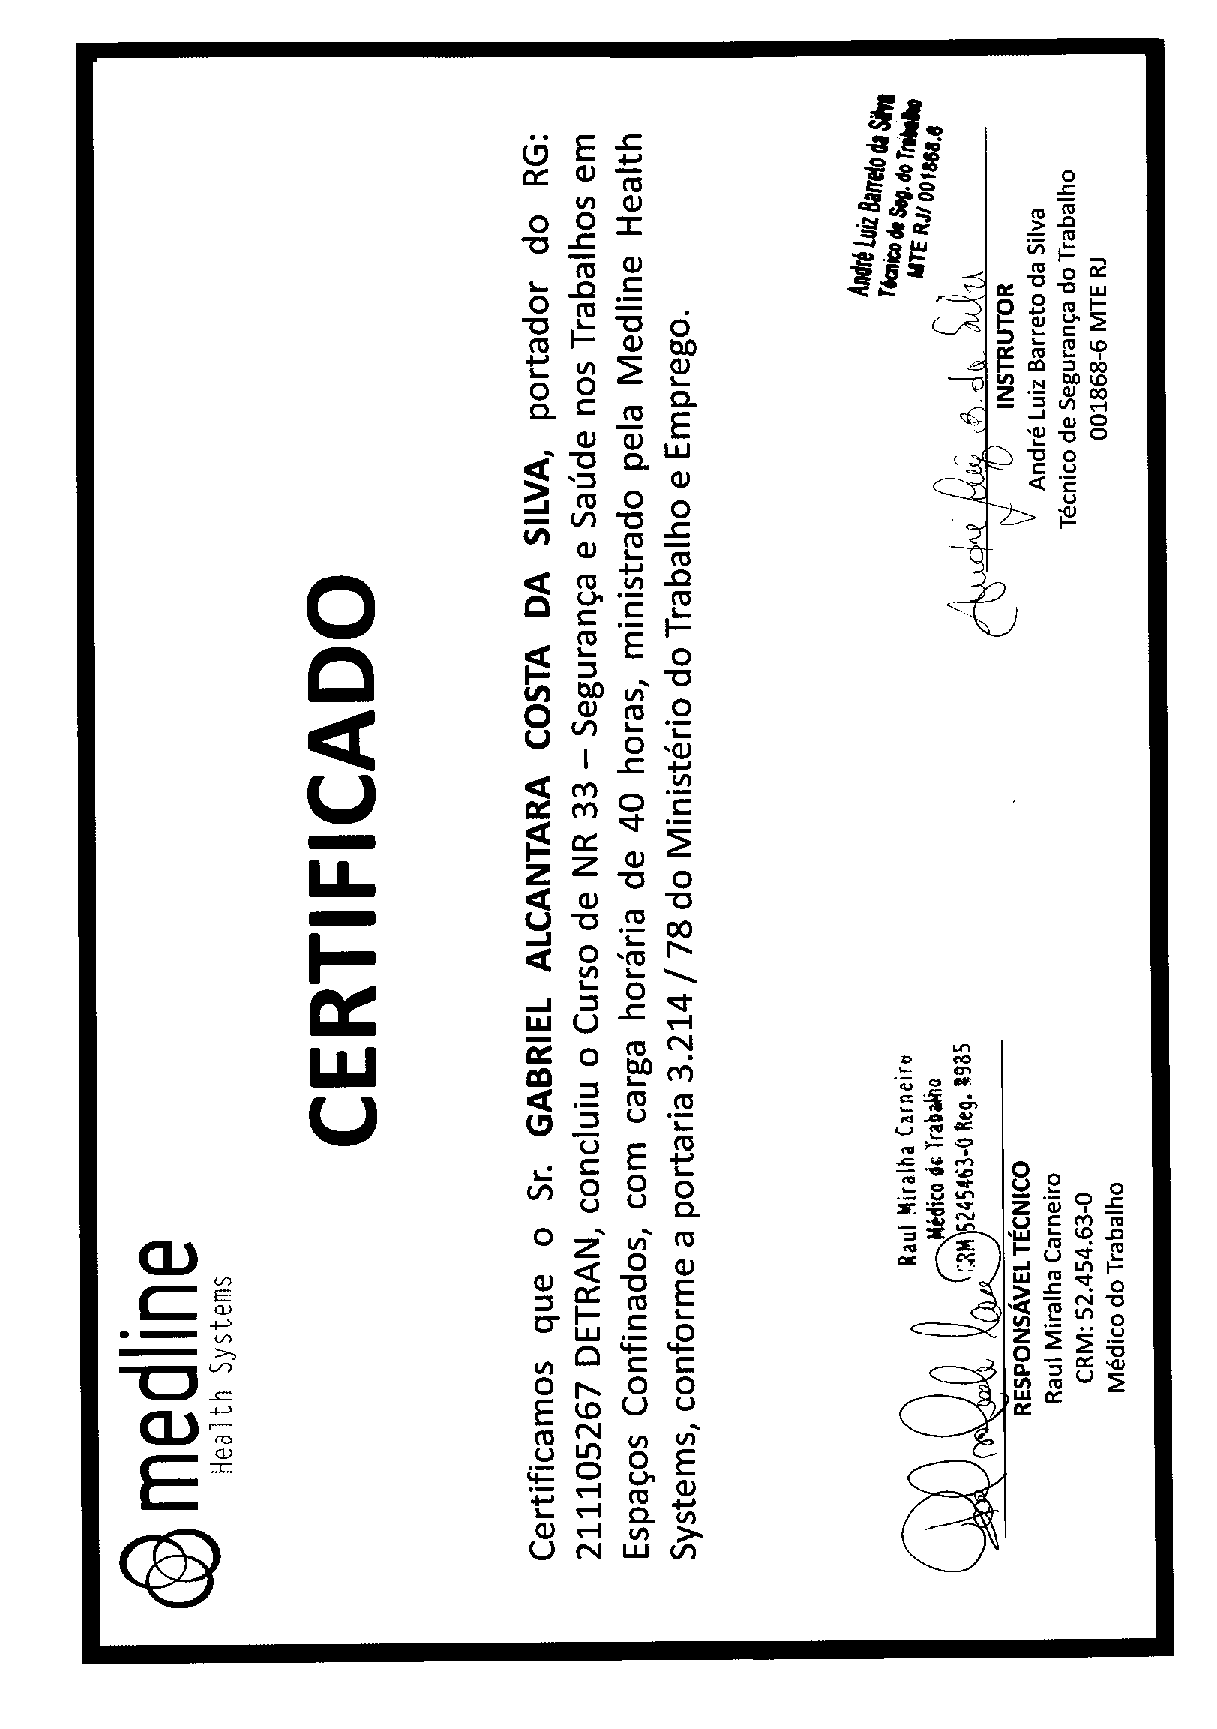
\includepdf[pages=1-]{pdfs/NR33}
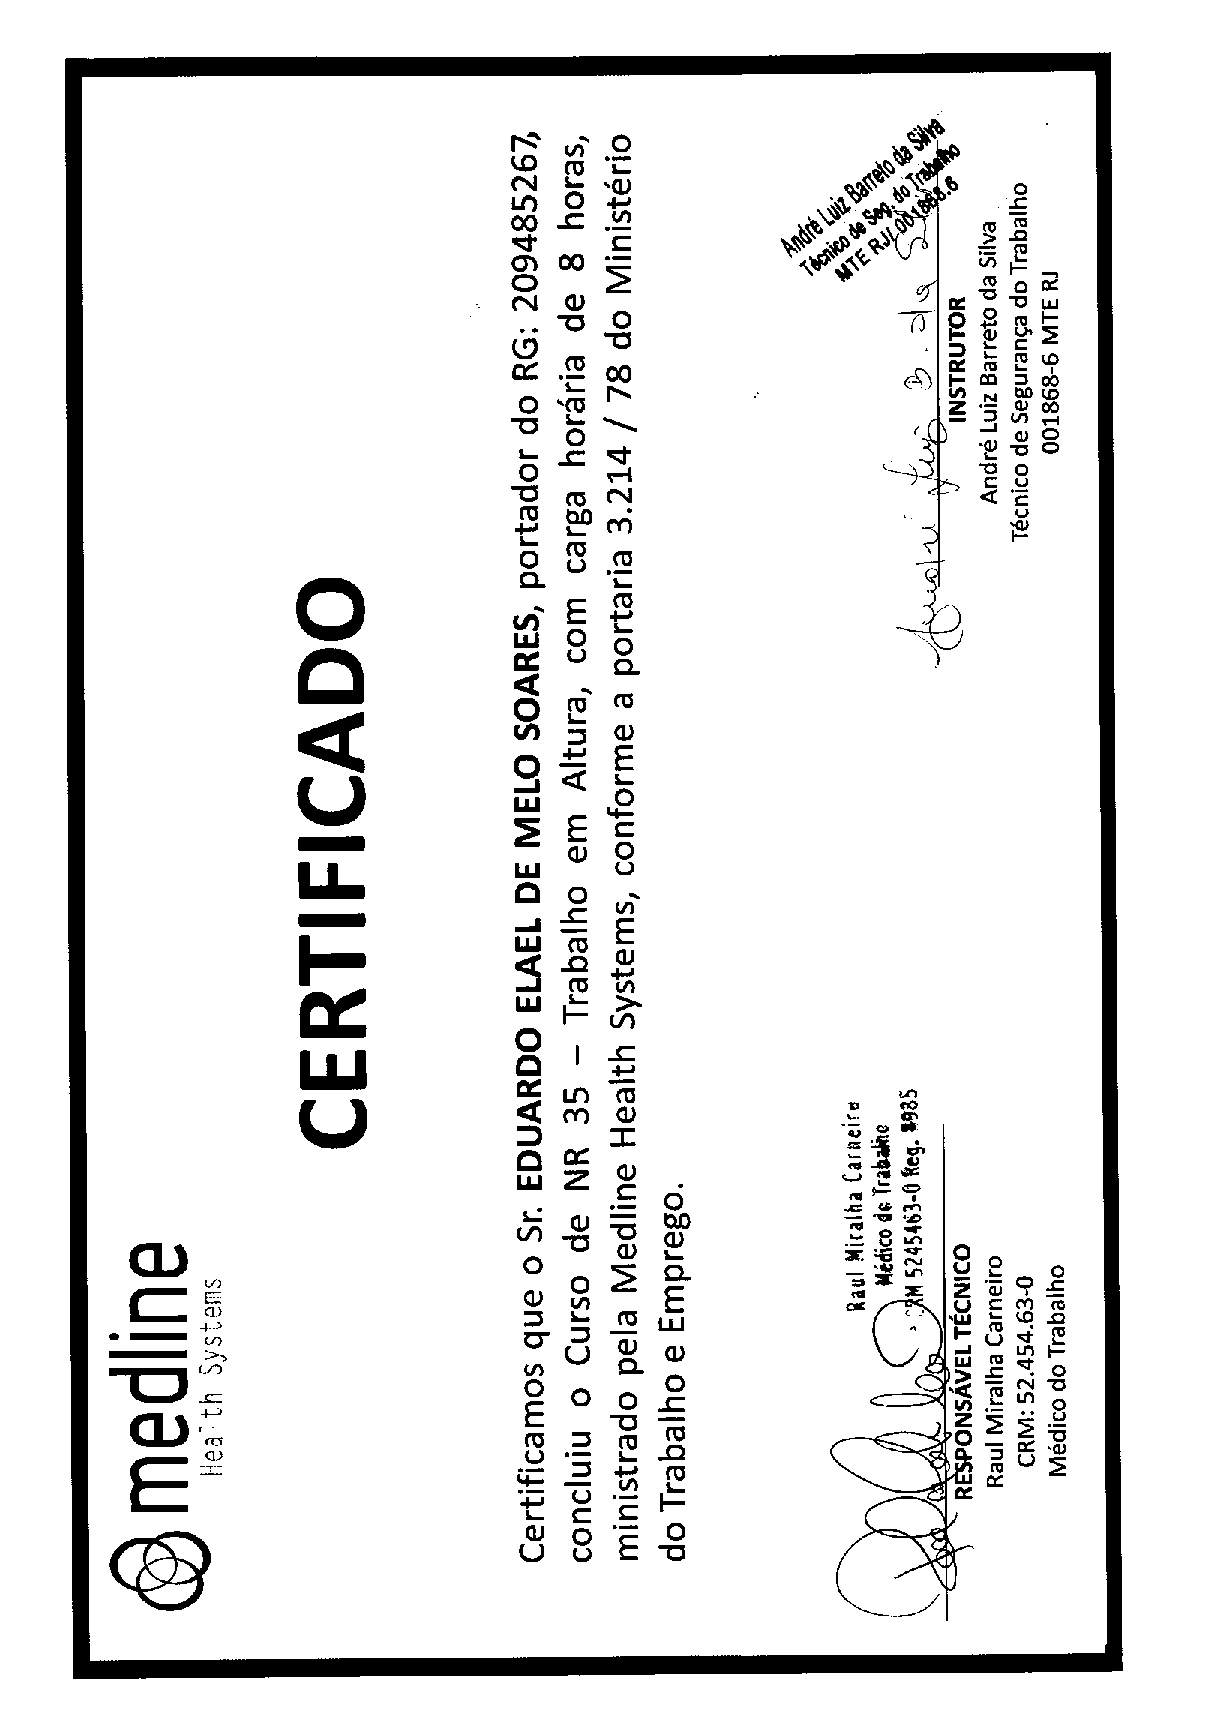
\includepdf[pages=1-]{pdfs/NR35}




% ---------------------------------------------------------------------------
% ---------------------------------------------------------------------------



 
 
% ---------------------------------------------------------------------------
% ---------------------------------------------------------------------------
%\chapter{Registros Fotográficos}
%\include{Nov2013}
%\include{solen}
%\include{LabOceano}
%\include{Jun2014}
%\include{Nov2014}
%\include{Jan2015}


% ---------------------------------------------------------------------------
% ---------------------------------------------------------------------------


% ---------------------------------------------------------------------------
% ---------------------------------------------------------------------------

%\chapter{Justificativa das alterações das informações relacionadas ao projeto
%base do XML inicial e a composição do XML final}
%\include{justificativaXML}

\standardchapterstyle   
\end{document}